\newcommand{\Versione}{1.0}%Versione Finale
\newcommand{\Data}{2013-01-21}%Data di creazione
%\newcommand{\TipoDocumento}{Relazione finale sullo stage}

\documentclass[a4paper]{article}
\usepackage[utf8x]{inputenc}
\usepackage[italian]{babel}
\usepackage{fancyhdr}
%%pacchetto per il float delle immagini
\usepackage{float}
\usepackage{sidecap,caption}
\usepackage{eurofont}
\usepackage{lastpage}
\usepackage{graphicx}
%\usepackage{fullpage}
\usepackage{setspace}
\usepackage{textcomp}
\usepackage{booktabs}
\usepackage{color}
\usepackage{lscape}
\usepackage{hyperref}
\hypersetup{colorlinks=true, linkcolor=blue, anchorcolor=red, urlcolor=blue}
\usepackage{longtable}
\usepackage{tabularx}
\usepackage{abstract}
\usepackage{appendix}
\usepackage{multicol}
\usepackage{bmpsize}
%%%%%%%%%%%%%%%needed for glossario%%%%%%%%%
%\usepackage{guit}

%\usepackage[acronym]{glossaries}
%\newglossaryentry{parola}{name=parola,description={Si spiega da sé}}
%\newacronym{guit}{\GuIT{}}{Gruppo Utilizzatori Italiani di \TeX{}}
%\addto\captionsitalian{\renewcommand{\glossaryname}{Glossario}}
%\makeglossaries
%%%%%%%%%%%%%%%%%%%%%%%%%fine need glossario
%%%%%%%%%%%glossario prova 2
\usepackage{glossaries}
\addto\captionsitalian{\renewcommand{\glossaryname}{Glossario}}
\newglossaryentry{prova}{name=prova, description={parole a caso}}
\newglossaryentry{dematerializzazione} {name=dematerializzazione, description={processo che ha come obiettivo ultimo la creazione di un flusso di documenti digitali aventi pieno valore giuridico, che vada prima ad affiancare e poi, sul lungo periodo, a sostituire la normale documentazione cartacea presente negli archivi di qualunque attività pubblica o privata.}}
\makeglossaries
%%%%%%%%%%%%%% fine glossario prova 2
\usepackage[all]{hypcap}
\oddsidemargin=.15in
\evensidemargin=.15in
\textwidth=6in
%\topmargin=-.5in
\parindent=0in
%\headheight=1in
\pagestyle{fancy}
\lhead{
\bfseries {\Large \TipoDocumento}\\
\bfseries Versione: \Versione\\
}
\chead{}
\lhead{
%\includegraphics[scale=0.455]{../Logo&Header/SEVENTECH2.png}
}
%\lfoot{\bfseries \TipoDocumento{} v\Versione}
\cfoot{}
\rfoot{\thepage\ of \mypageref{LastPage}}
\newcommand*{\mypageref}[1]{
\hypersetup{linkcolor=black}\pageref{#1}\hypersetup{linkcolor=black}}
%\userpackage{lipsum}
\renewcommand{\footrulewidth}{0.4pt}
%\newcommand{\numref}[1]{\textsl{\nameref{#1} (\ref{#1})}}
%\newcommand{\NomeGruppo}{SevenTech}
%\newcommand{\Progetto}{''3DMob: Grafica 3D su device mobili''}
%\newcommand{\Prop}{Mentis s.r.l.}
%\newcommand{\Glossario}{Al fine di evitare incomprensioni dovute a possibili ambiguità del linguaggio, dei termini e acronimi utilizzati nei documenti, viene allegato il glossario contenuto nel file \emph{Glossario\_{}vX.Y.pdf}.
%Saranno in esso definiti e descritti tutti i termini marcati da una \underline{sottolineatura} nella documentazione fornita.}

%\newcommand{\Prodotto}{

%Il prodotto denominato 3DMob ha lo scopo di fornire un \underline{applicativo} in grado di interpretare \underline{oggetti 3D} a partire dai \underline{formati} \underline{3DS} o \underline{OBJ} e relativo file \underline{MTL}, permettendo all'\underline{utente} di applicare modifiche alla \underline{scena 3D} e di visualizzarne l'anteprima. Il prodotto dovrà successivamente consentire l'\underline{esportazione} del modello 3D nel \underline{formato} \underline{JSON} o \underline{XML}, in modo tale che sia immediatamente compatibile con le \underline{librerie} grafiche \underline{\underline{OpenGL} ES} 2.0, utilizzate nei \underline{device mobili}.
%  Tale formato dovrà essere conforme ai limiti impliciti delle \underline{librerie} grafiche \underline{OpenGL ES} 2.0, in modo che i file esportati possano essere immediatamente utilizzabili nei \underline{device mobili} che supportano tali librerie.

%}
\begin{document}
%\thispagestyle{empty}
%\begin{center}%\centerline{
%\includegraphics[scale=1.05]{../Logo&Header/logo_principale.png}}
%{\href{mailto:grupposwe2013@gmail.com}{\color[rgb]{0.39,0.37,0.38}grupposwe2013@gmail.com}}\\ [3pc]
%{\Huge {3DMob: Grafica 3D su device mobili}}\\[.5pc]
%\underline{\hspace{6in}}\\[3pc]
%{\Huge {\TipoDocumento}}\\[1pc]
%{\emph{Versione \Versione}}\\
%\end{center}
%\vspace{.3in}
\begin{titlepage}
 
\begin{center}
 
% Upper part of the page

\includegraphics[scale=.5]{logoBlack.png}
 
\textsc{\LARGE Università degli Studi di Padova}\\[1.5cm]
 
\textsc{\Large Dipartimento di Matematica\\[0.2cm] Corso di Laurea in Informatica}\\[0.8cm]
  
% Title
\\[0.8cm]{\Huge \doublespacing \bfseries \begin{spacing}{1}{Classificazione firme statiche utilizzando i Hidden~Markov~Models}\end{spacing}}
\\[2cm]

% Author and supervisor
\begin{minipage}{0.4\textwidth}
\begin{flushleft} \large
\emph{Relatore:} \\
Ch.mo Prof. Tullio \textsc{Vardanega}
\end{flushleft}
\end{minipage}
\begin{minipage}{0.4\textwidth}
\begin{flushright} \large
\emph{Laureando:}\\
Alexandru \textsc{Prigoreanu 1004887}
\end{flushright}
\end{minipage}
 
\vfill
 
% Bottom of the page
{\large Anno accademico 2012/2013}
 
\end{center}
 
\end{titlepage}


%\vspace{.4in}

%TESTO DEL SOMMARIO
\null\vspace{2.0in}
\begin{abstract}
La presente relazione ha come scopo la descrizione dell'attività di \emph{stage}, svolta dal sottoscritto, nel periodo settembre-ottobre 2013 presso l'azienda Corvallis. Il primo capitolo descrive l'azienda ospitante. Il secondo capitolo espone le motivazioni e gli obiettivi del progetto di \emph{stage}. Il terzo capitolo illustra in modo approfondito le attività effettuate per raggiungere gli obiettivi prefissati. Il quarto ed ultimo capitolo riporta una valutazione a posteriori sul lavoro svolto, sulle conoscenze acquisite e sulla distanza tra le conoscenze richieste e le conoscenze possedute.
\end{abstract}
\vspace{\fill}
%
\newpage
\section*{Convenzioni tipografiche}
Al fine di migliorare la leggibilità e la chiarezza dei contenuti esposti sono state adottate le seguenti convenzioni tipografiche:
\begin{itemize}
\item Problema : pdf ci sono i link andata e ritorno ... ma stampato no!, definisci convenzioni che valgono per entrambe le situazioni, per la legge dell'accessibilità generale il colore non deve veicolare informazioni
\item \emph{corsivo} per i termini in lingua diversa dall'italiano
\item \emph{corsivo} per i nomi propri che individuano tecnologie
\end{itemize}

\newpage
\tableofcontents

\newpage

\listoftables
\listoffigures

\newpage

\section{Dominio applicativo}\\
\label{1.0}
La prima parte di questa relazione si prefigge di presentare al lettore il contesto di lavoro dell'azienda ospitante il progetto di \emph{stage}. Inizialmente descrivo brevemente l'azienda. A seguire effettuo una panoramica sui prodotti e servizi che essa offre e sui clienti che cerca di soddisfare. Infine elenco alcune delle tecnologie di appoggio allo sviluppo software e i processi interni di quest'ultimo.

\subsection{Azienda}
\label{1.1}

\begin{figure}[h!]
\centering

\includegraphics[scale=0.75]{../Logo&Header/logoCorvallis.png}
\caption{ Logo azienda Corvallis}
\end{figure}

Corvallis S.p.A. (http://www.corvallis.it/) è una società italiana presente nel settore dell’\emph{Information Technology}. Essa applica le sue competenze funzionali, tecnologiche e di processo, acquisite in quasi trenta anni di operatività, in 4 settori strategici per il mondo finance:
\begin{itemize}

\item risparmio gestito e crediti;
\item \emph{document management};
\item area compliance;
\item evoluzione tecnologica.\\
\end{itemize}

Corvallis fornisce prodotti e servizi a clienti appartenenti all'ambito finanziario (banche e assicurazioni), industria/servizi e Pubblica Amministrazione. In particolare, Corvallis effettua attività di progettazione e sviluppo software, di fornitura di prodotti software propri e di terzi, di manutenzione e assistenza tecnica, di consulenza.

Il Gruppo Corvallis è composto da più di 600 risorse, tra dipendenti e collaboratori, distribuite in 13 sedi operative nel territorio italiano.

\subsection{Prodotti e clienti}
\label{1.2}
\subsubsection{Banche}
\label{1.2.1}
Corvallis opera da molti anni con i principali istituti di credito e società prodotto. Le aree di competenza sviluppate riguardano:
\begin{itemize}
\item Risparmio Gestito;
\item Finanza;
\item Crediti;
\item Compliance;
\item \emph{Governance};
\item Sistemi di Pagamento;
\item \emph{Document Management}.\\
\end{itemize}
%Esempi di prodotti in questo ambito:
%\begin{itemize}
%\item Antifrode Carte Pagamento, Soluzione per la prevenzione delle frodi sulle carte di pagamento;
%\item RG - GeDoFi, Sistema di Gestione Documentale per Banca Depositaria;
%\item FIRME - CSIGNgra, Tecnologia di riconoscimento e cattura della firma biometrica.
%\end{itemize}
\subsubsection{Assicurazioni}
\label{1.2.2}
Corvallis può effettuare \emph{outsourcing} nelle compagnie Assicurative per i processi Vita e Danni (IT e \emph{back office}). L'offerta verso le compagnie assicuratrici riguarda le seguenti aree:
\begin{itemize}
\item Sistema Portafoglio Vita e Danni;
\item Sistemi di agenzia;
\item Sistemi sinistri;
\item Compliance;
\item \emph{Governance};
\item Servizi di \emph{Back Office};
\item \emph{Outsourcing};
\item \emph{Document Management}.
\end{itemize}

\subsubsection{Industria e servizi}
\label{1.2.3}
I clienti di Corvallis sono alcune industrie e imprese appartenenti a differenti settori: \emph{Oil~\&~Gas}, \emph{Engineering}, \emph{Construction}, \emph{Aerospace~\&~Defense}, Telco, Media. Corvallis possiede competenze anche nell'ambito del \emph{Project~\&~Portfolio Management}. Inoltre svolge erogazione di servizi di supporto specialistico relativo a prodotti leader di mercato tra i quali Cognos, Qlikview, Hyperion, Business~Object e IrionDQ.
\subsubsection{Pubblica Amministrazione}
\label{1.2.4}
Corvallis offre soluzioni e servizi alle pubbliche amministrazioni. Alcune di queste riguardano:
\begin{itemize}
\item Tributi e fiscalità per gli enti locali;
\item Sistemi informativi territoriali e catastali, \emph{GIS}, \emph{Digital Mapping} e cartografia;
\item \emph{Document Management};
\item Sistemi Informativi per la catalogazione, conservazione e la tutela dei Beni Culturali.\\
\end{itemize}
%Esempi di prodotti in questo ambito:
%\begin{itemize}
%\item AML - WINTAR, prodotto per la gestione dell'Archivio Unico Informatico
%\item AML - Agenzia delle Entrate, prodotto per la gestione delle segnalazioni di vigilanza verso l'Agenzia delle Entrate.
%\end{itemize}
\subsubsection{\emph{Know Your Customer} (\emph{KYC})}
\label{1.2.5}
\emph{Know Your Customer} è un prodotto sviluppato dall'azienda Corvallis per soddisfare i requisiti normativi richiesti dalla direttiva Cee in materia di Antiriciclaggio. \'{E} un software utile alle banche e alle assicurazioni poiché permette di tenere sotto controllo la segnalazione di operazioni sospette previste dalla normativa. Il prodotto si compone di sette moduli integrabili e flessibili:
\begin{itemize}
\item \emph{Repository}, modulo che archivia in un unico ambiente tutte le informazioni relative al cliente e la sua operatività, necessarie a soddisfare le diverse richieste imposte dalla normativa;
\item \emph{Classifier}, modulo che racchiude una generale profilatura del Cliente rispetto ad un numero non prefissato di dimensioni, indipendenti tra loro ma con la condivisione di dati e funzioni;
\item \emph{Integrator}, modulo di integrazione delle fonti esterne, fornisce tutte le funzioni richieste per l'import e l'aggregazione delle liste sia pubbliche che private (ad esempio Persone Politicamente Esposte);
\item \emph{Expansion}, modulo basato su logiche di intelligenza artificiale, soddisfa l'esigenza di ricerche di ricorrenze di dati, presenti nelle liste pubbliche, nei database interni, nei database forniti da \emph{info providers}, oppure nei dati acquisiti tramite il modulo \emph{Integrator};
\item \emph{Control}, modulo che presidia l'analisi dell'operatività della clientela considerando i dati anagrafici, di rapporto e di movimentazione, generando degli aggregati statistici da analizzare;
\item Monitor, modulo che  propone un'interfaccia utente per visualizzare e analizzare gli \emph{"alert"} generati dai moduli \emph{Classifier}, \emph{Expansion} e \emph{Control};
\item \emph{Configurator}, modulo che permette di assicurare un approccio flessibile ed efficiente che può essere facilmente modificato rispondendo ai cambiamenti repentini delle regole internazionali o interne all'organizzazione. Il modulo governa le parametrizzazioni delle altre componenti del prodotto \emph{KYC}.
\end{itemize}
Il software è stato scritto in \emph{Java} utilizzando il \emph{framework} aziendale.
\subsection{Tecnologie}
\label{1.3}
Seguono alcune delle tecnologie impiegate nello sviluppo software.

I linguaggi di programmazione più utilizzati sono \emph{Java} e \emph{Cobol}.

Il sistema di versionamento in uso è il \emph{Concurrent Versions System} (\emph{CVS}).

Alcuni dei database utilizzati sono: \emph{DB2}, \emph{Oracle}, \emph{MS SQL}, \emph{PostgreSQL}.

I \emph{framework} maggiormente utilizzati sono \emph{JBoss} e \emph{JWolf}. \emph{JWolf} è stato creato dall'azienda stessa.\'{E} un \emph{framework} per lo sviluppo di applicazioni su tecnologia \emph{Java} multipiattaforma e multicanale e racchiude le \emph{best practices} dell'architettura {Service Oriented Architecture} (\gls{Service Oriented Architecture}).

L'ambiente di sviluppo per \emph{Java} è \emph{Eclipse}.\\

In figura 2 possiamo vedere uno schema riassuntivo di alcune delle tecnologie in uso.
\begin{figure}[H]
\centering
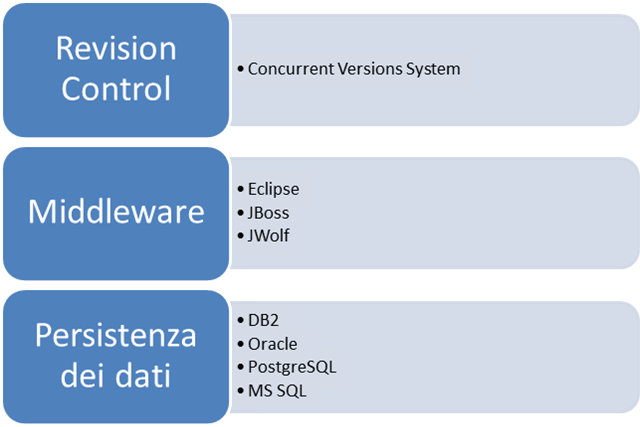
\includegraphics[scale=0.55]{../Logo&Header/tecnologieUsate.png}
\caption{Tecnologie in uso}
\end{figure}


\subsection{Processi interni}
\label{1.4}
Le fasi di sviluppo di un progetto sono costituite da:
\begin{itemize}
\item Coordinamento e Riunioni.
In questa fase vengono pianificate tutte le attività necessarie allo svolgimento del progetto. Gli incontri con i clienti hanno come scopo una efficiente trasmissione di informazioni;
\item Analisi dei requisiti.
L'output dell'attività di analisi è un documento in cui vengono racchiusi tutti i requisiti funzionali, qualitativi, prestazionali e dichiarativi dei quali il prodotto finale dovrà garantirne il soddisfacimento. Il documento serve da input per la fase di progettazione;
\item Progettazione.
Nella fase di progettazione si definiscono le specifiche tecniche delle funzionalità da realizzare. Il risultato di questa fase è il documento di Specifiche Tecniche di Progettazione;
\item Sviluppo.
\'{E} lo stadio esecutivo del progetto con il quale si realizzano i moduli software previsti dal disegno applicativo. In questa fase vengono effettuati test di unità;
\item Test funzionali e di sistema.
I test funzionali hanno lo scopo di verificare che i moduli realizzati durante la fase di codifica rispettino quanto fissato dai requisiti iniziali. Il test di sistema valida il prodotto nella sua interezza;
\item Collaudo con il cliente.
Si tratta di un test di sistema effettuato su un ambiente del cliente e con dati di prova forniti dallo stesso. L'output di questa attività è un verbale che racconta l'esito del collaudo;
\item Documentazione di prodotto.
Questa fase prevede la stesura dei Manuali di Prodotto relativi al software realizzato;\\
\end{itemize}

L'output di ogni fase viene verificato e, se conforme agli standard di qualità dell'azienda, approvato. Altrimenti dovranno essere indicate delle misure correttive per i problemi individuati.\\

In figura 3 vediamo un resoconto delle fasi necessarie allo sviluppo software.
\begin{figure}[H]
\centering
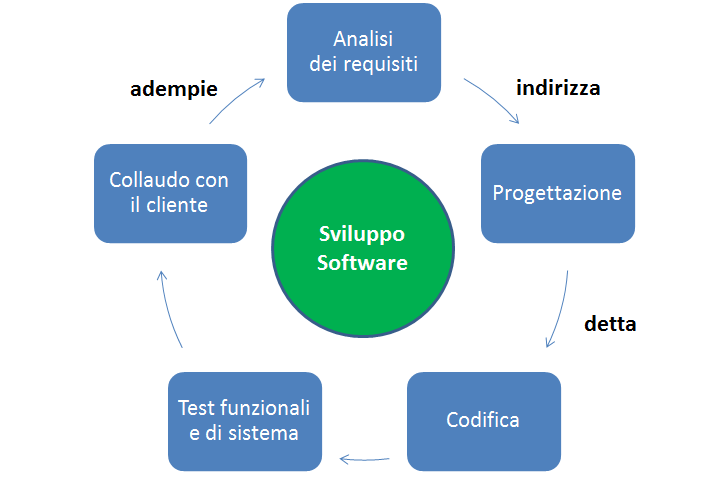
\includegraphics[scale=0.55]{../Logo&Header/sviluppoSoftware.png}
\caption{ Sviluppo Software, ciclo di vita}
\end{figure}

\newpage
\newpage

\section{Progetto aziendale}
\label{2.0}
Questo capitolo ha lo scopo di mostrare al lettore l'ambito in cui si colloca il progetto di \emph{stage} proposto dall'azienda Corvallis. Inizialmente presento i motivi che hanno portato alla nascita del progetto. A seguire effettuo una panoramica sulla classificazione delle firme statiche. In seguito descrivo il prototipo/classificatore preesistente al progetto di \emph{stage}. Infine illustro gli obiettivi, le aspettative e i vincoli del progetto aziendale a cui ho preso parte.\\\\
Visti i notevoli vantaggi in termini di incremento dell'efficienza e di riduzione dei costi che la \gls{dematerializzazione} garantisce (risparmio relativo ai costi di stampa, acquisto e manutenzione delle stampanti), nell'ambito delle nuove normative alle banche sarà concesso lo scambio di immagini degli assegni bancari. 

In base a questa premessa l'azienda Corvallis ha intuito che il core di un'applicazione bancaria che accetta lo scambio di immagini degli assegni bancari sarà un classificatore di firme statiche accurato, robusto e affidabile. Conseguentemente ha implementato un prototipo per la classificazione di firme statiche.

\subsection{Introduzione alla classificazione di firme statiche}
\label{2.1}
La firma è un tratto comportamentale di un individuo e costituisce una particolare classe di scrittura dove lettere o parole possono essere non distinguibili. \'{E} considerata un elemento distintivo avente caratteristiche uniche e personali. Accertare in maniera chiara ed univoca il sottoscrittore di un documento avente forza legale (in questo caso assegni bancari) è di fondamentale importanza. Infatti il destinatario deve poter identificare l'identità del mittente (autenticità) e il mittente non deve poter disconoscere un documento da lui firmato (non ripudio). Nasce quindi l'esigenza di distinguere tra firme false e firme autentiche.\\\\
Le difficoltà principali nel classificare le firme autografe sono dovute alle variazioni intrapersonali: le firme di una persona possiedono grande variabilità, dovuta allo stato emotivo dei sottoscrittori oppure alla posizione di raccolta, e di conseguenza, se confrontassimo due esemplari di firma di un firmatario questi non sarebbero identici. Invece l'agevolazione cardinale sta nel fatto che le firme di persone diverse manifestano caratteristiche elementari distinte.\\\\
A seconda del hardware front-end, un sistema di verifica della firma (\emph{signature verification system}) può essere etichettato come \emph{offline} o \emph{online}. Nei sistemi \emph{offline} la verifica della firma avviene dopo la sottoscrizione della firma. Le uniche informazioni che si possiedono sono di natura statica: l'immagine della firma autografa del sottoscrivente. Al contrario, nei sistemi online, le firme vengono acquisite tramite un dispositivo elettronico (tavoletta grafica) oppure con una penna speciale, capace di memorizzare una sequenza di punti che descrivono velocità, pressione, ritmo, accelerazione e movimento effettuati dal sottoscrittore, non solo l'immagine statica.

\subsubsection{Valutazione delle performance}
\label{2.1.1}
La performance di un sistema di verifica della firma si calcola in base alla percentuale di errori che esso commette nel classificare le firme. Esistono due tipi di errori. Questi vengono riassunti dai seguenti indici:
\begin{itemize}
\item \emph{False Acceptance Rate} (\emph{FAR}), indice di accettazione dei falsi, ossia percentuale delle firme false classificate come genuine;
\[FAR =
\frac{nr.\ falsi\ accettati}{nr.\ falsi\ totali}
\]
\item \emph{False Rejection Rate} (\emph{FRR}), indice di rifiuto dei genuini, ossia percentuale delle firme genuine classificate come false.
\[FRR =
\frac{nr.\ genuini\ rifiutati}{nr.\ genuini\ totali}
\]
\end{itemize}
Purtroppo i due indici sono inversamente proporzionali: a una diminuzione del \emph{FAR} corrisponde un aumento del \emph{FRR} e viceversa a una diminuzione del \emph{FRR} corrisponde un aumento del \emph{FAR}. \'{E} evidente quindi che si deve arrivare a un compromesso: minimizzare il \emph{FAR} conservando un valore tollerabile per il \emph{FRR}.

Se si eguagliano i due indici si è in presenza di un nuovo indice: \emph{Equal Error Rate} (\emph{EER}). L'\emph{EER} permette di paragonare in modo veloce l'accuratezza dei sistemi di verifica. In generale, più l'indice \emph{EER} è basso più il sistema è accurato.

Non sorprendentemente, grazie ai dati biometrici che i sistemi di verifica della firma online possiedono in più, essi sono più accurati e affidabili dei sistemi di verifica della firma statica.

\subsubsection{Tipi di falsificazione}
\label{2.1.2}
In letteratura sono stati individuati tre tipi di falsificazione a seconda del grado di preparazione del falsificatore sulla firma che sta cercando di riprodurre:
\begin{itemize}
\item falsificazioni casuali (\emph{random forgeries}), prodotte senza conoscere né il nome del firmatario né la forma della sua firma;
\item falsificazioni semplici (\emph{simple forgeries}), prodotte conoscendo il nome del firmatario ma senza avere un esempio della sua firma;
\item falsificazioni accurate (\emph{skilled forgeries}), prodotte dopo un allenamento con l'obiettivo di imitare la firma originale nel miglior modo possibile.
\end{itemize}
In figura 4 vediamo un esempio di firma genuina e degli esempi di falsificazione della stessa.
\begin{figure}[H]
\centering
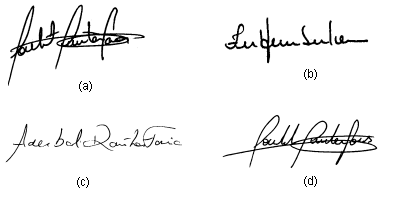
\includegraphics[scale=1.0]{../Logo&Header/esempiForged.png}
\caption{Tipi di falsificazioni:} (a) firma genuina; (b) falsificazione casuale;\\
(c) falsificazione semplice; (d) falsificazione accurata
\end{figure}

\subsubsection{Verifica della firma statica (\emph{offline signature verification})}
\label{2.1.3}
La verifica di firme statiche appartiene alla classe di problemi del \emph{pattern recognition} e un tipico sistema di \emph{pattern recognition} si compone dai seguenti step \cite{2698894}:
\begin{enumerate}
\item Acquisizione dati, cattura delle immagini firma;
\item \emph{Preprocessing}, per semplificare le operazioni successive minimizzando la perdita di informazioni;
\item Estrazione delle caratteristiche (\emph{feature extraction}), riduzione dei dati in input misurando solo determinate caratteristiche (\emph{feature}) o proprietà;
\item Classificazione (oppure fase di verifica), prendere una decisione (accettare o rifiutare) sulla base dell'adeguatezza dei valori ottenuti dalla fase di \emph{feature extraction}.
\end{enumerate}
In figura 5 vediamo il \emph{workflow} generale del processo di verifica della firma statica.
\begin{figure}[H]
\centering
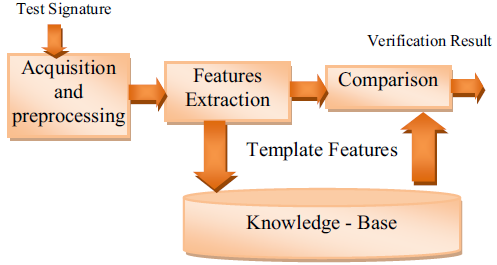
\includegraphics[scale=0.8]{../Logo&Header/generalProcess.png}
\caption{\emph{Workflow} dei sistemi di verifica della firma statica} Sorgente: \cite{4}
\end{figure}
\subsubsection*{Acquisizione dati}
\label{2.1.3.1}
Le immagini di firma vengono scannerizzate oppure vengono estratte da documenti \emph{PDF}.
\subsubsection*{\emph{Preprocessing}}
\label{2.1.3.2}
Il \emph{preprocessing} della firma è uno step fondamentale necessario a migliorare l'accuratezza dell'estrazione delle caratterisitche e della classificazione. Lo scopo della fase di \emph{preprocessing} è quello di standardizzare le firme e renderle pronte per la fase di \emph{feature extraction}.\\ Di seguito elenco alcune delle operazioni di \emph{preprocessing} più utilizzate:
\begin{itemize}
\item Estrazione della firma (\emph{signature extraction});
\item Ritaglio (\emph{cropping}), l'immagine viene ridotta al rettangolo che circoscrive la firma;
\item Ridimensionamento (\emph{resizing}), l'immagine della firma viene ridimensionata;
\item Binarizzazione (\emph{binarization}), conversione da colore a scala di grigi e infine a bianco-nero (binario);
\item Assottigliamento (\emph{thinning}), assottigliamento del tratto della firma a un pixel per uniformare lo spessore;
\end{itemize}
Un'errata scelta degli algoritmi di \emph{preprocessing} può comportare una considerevole perdita di informazione.

\subsubsection*{Estrazione delle \emph{features}}
\label{2.1.3.3}
Il successo di un sistema di verifica della firma dipende fortemente dalla fase di Estrazione delle \emph{features}. Un metodo ideale di \emph{feature extraction} prevede l'estrazione di quelle caratteristiche che minimizzano le variazioni intrapersonali presenti nelle firme di un sottoscrittore e massimizzano le variazioni interpersonali presenti nelle firme di due sottoscrittori distinti\cite{2}.\\\\
A seconda della facilità con la quale si possono imitare, le \emph{feature} possono essere classificate in \emph{feature} statiche o \emph{feature} pseudo-dinamiche. La prima categoria contiene caratteristiche percettive e quindi facili da imitare, mentre la seconda categoria contiene caratteristiche poco intuitive e quindi di difficile imitazione\cite{3}.
Segue un elenco stringato delle \emph{features} più utilizzate in letteratura.\\
\emph{Features} statiche:
\begin{itemize}
\item \emph{Calibre}, valore che individua il rapporto tra altezza e larghezza della firma;
\item \emph{Proportion}, si riferisce alle simmetrie presenti nell'immagine
\item \emph{Spacing}, valore che individua il numero di blocchi che compongono la firma, se non vi sono spaziature questo valore è uguale a 1;
\item \emph{Base behavior}, descrive l'angolo di inclinazione della firma in base a un'immaginaria linea orizzontale.
\end{itemize}
\emph{Features} pseudo-dinamiche:
\begin{itemize}
\item \emph{Density of pixels}, descrive la larghezza dei tratti, viene considerata "pressione apparente";
\item \emph{Distribution of pixels}, descrive il numero di pixel neri presenti in uno spazio;
\item \emph{Slant}, individua informazioni riguardo all'inclinazione del tratto in considerazione;
\item \emph{Form}, individua informazioni riguardo alla forma del tratto in considerazione;
\end{itemize}
Un'ulteriore suddivisione delle \emph{features} è dovuta alla segmentazione. In presenza di un'immagine firma segmentata le \emph{features} possono essere globali (riguardano l'immagine nella sua interezza) o locali (riguardano determinate parti dell'immagine).\\\\
In figura 6 vediamo la panoramica delle \emph{features} sopra elencate.
%prima era scritto \begin{figure}[h!] per il float default immagini?
\begin{figure}[H]
\centering
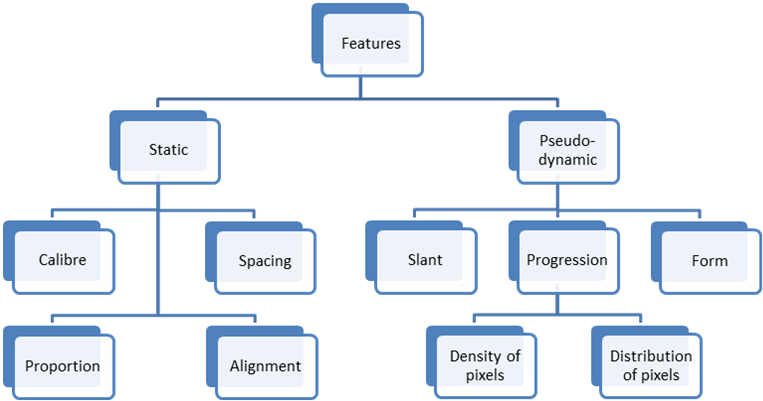
\includegraphics[scale=0.7]{../Logo&Header/featuresStaticPseudoD.png}
\caption{Features statiche e features pseudo-dinamiche}
\end{figure}
\subsubsection*{Classificazione}
\label{2.1.3.4}
L'ultimo step nel processo di verifica dei sistemi \emph{offline} decide se la firma presa in considerazione è genuina o falsa.\\
In letteratura esistono diversi tipi di approcci al problema della classificazione di firme statiche.\\\\
In figura 7 riporto un grafico riassuntivo degli approcci più utilizzati.\\
\begin{figure}[H]
\centering
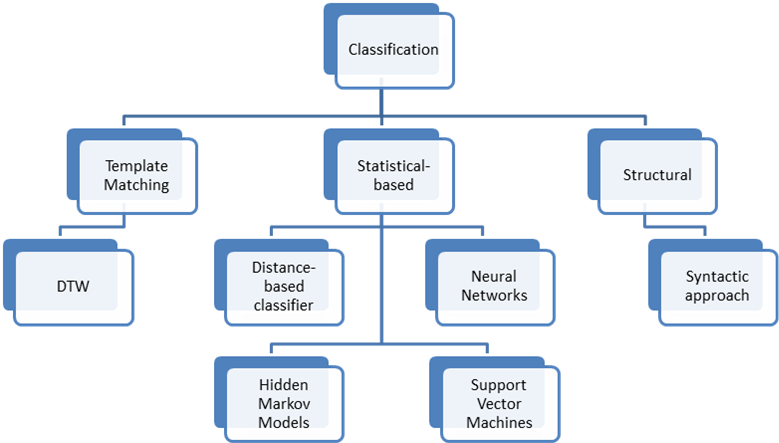
\includegraphics[scale=0.7]{../Logo&Header/classificatori.png}
\caption{Panoramica metodi di classificazione}
\end{figure}
Poiché alcuni dei prossimi argomenti di questa relazione trattano i classificatori di tipo \emph{Statistical-based}, né spiego la logica.
\subsubsection*{Classificatori \emph{Statistical-based}}
\label{2.1.3.5}
Nei classificatori di tipo \emph{Statistical-based} la conoscenza statistica viene utilizzata per usufruire di nozioni come la relazione, la deviazione, tra due o più item per trovare qualche specifica correlazione tra essi. Nei sistemi di verifica della firma, la firma media (\emph{template}/\emph{pattern}) viene elaborata a partire da firme collezionate precedentemente (nella fase di training). Questa viene salvata nella "base di conoscenza" e quando si ha in input una firma da classificare viene utilizzato il concetto di correlazione per calcolare la distanza tra la firma da verificare e la firma media per poi decidere se accettarla o rifiutarla.\\\\
Nella prossima sezione descrivo il classificatore di firme statiche implementato dall'azienda Corvallis prima del progetto di \emph{stage}.
\subsubsection{Prototipo preesistente}
\label{2.1.4}
Il classificatore di firme statiche, implementato dall'azienda, fa parte della categoria \emph{Statistical-based}. In particolare è un classificatore di tipo \emph{Distance-based}.\\\\
Il prototipo è in grado di estrarre 21 \emph{features}.
Il sistema viene addestrato utilizzando un database di firme. Per ciascun sottoscrittore, un vettore contenente il baricentro di ogni \emph{feature} (\emph{centroid feature vector}) viene calcolato utilizzando gli esemplari di firma genuini. Il vettore baricentro costituisce il \emph{template} delle firme del firmatario. In fase di verifica, per misurare la distanza tra la firma \emph{template} e la firma da testare, viene adoperata la distanza Euclidea nello spazio delle \emph{features}.\\
La particolarità di questo sistema sta nel fatto che, per classificare una firma, non si basa soltanto sulla distanza Euclidea ma anche su un meccanismo dei pesi. Si assegna una peso ad ogni \emph{feature} in base alla variabilità intrapersonale che essa assume tra i prototipi firma di un sottoscrittore. Questa meccanica è descritta meglio nelle sezioni a seguire.\\\\
In figura 8 segue uno schema riassuntivo dei processi interni al classificatore.
\begin{figure}[H]
\centering
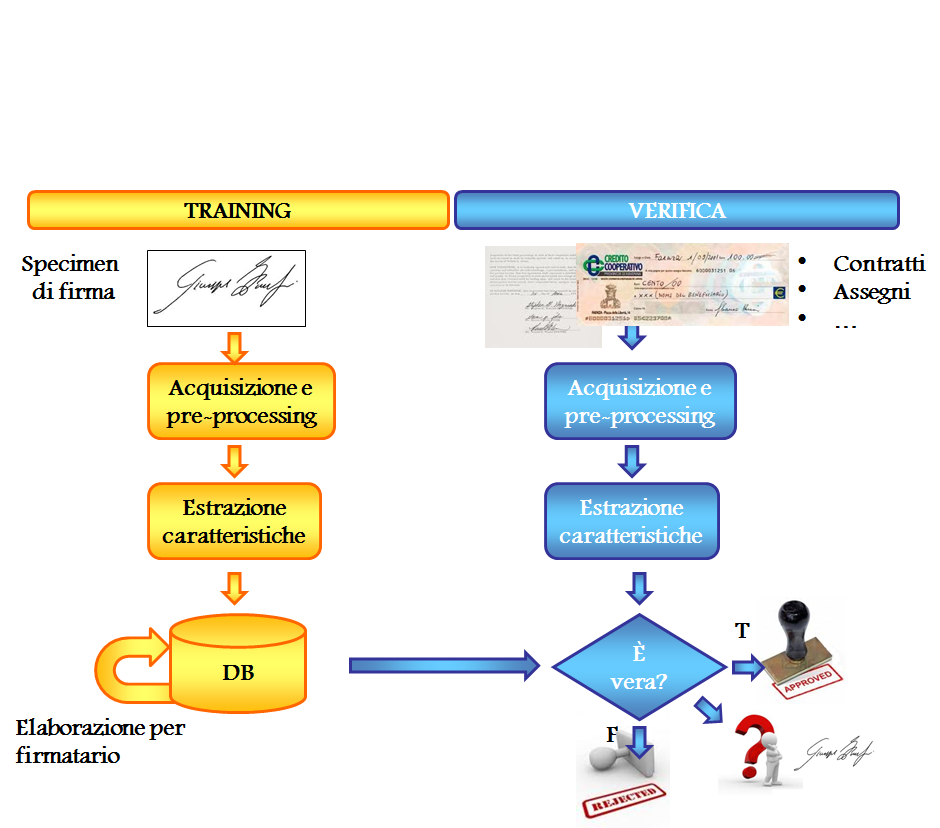
\includegraphics[scale=0.6]{../Logo&Header/processoPrototipoPrees.png}
\caption{Il processo}Sorgente:Corvallis
\end{figure}

\subsubsection*{Fase di training}
\label{2.1.4.1}
Il training prende in input N prototipi di firma genuina, una lista di \emph{feature} da estrarre e i \emph{preprocessing} necessari ad ogni \emph{feature}. Restituisce in output un file contenente quattro attributi per \emph{feature}, utili in fase di verifica:
\begin{itemize}
\item \emph{average}, la media di una \emph{feature} è data dalla somma dei valori che tale \emph{feature} assume negli N prototipi diviso N:
\[Faverage =
\frac{\sum\limits_{i=1}^N FValPrototipoI}{N}
\]
\item \emph{threshold}, la soglia di una \emph{feature} è data dal massimo valore tra la massima distanza del valore della \emph{feature} dalla media e il 10\% della media:
\[Fthreshold = 
\max \lbrack \max ( |FValPrototipoI - Faverage| ) , ( Faverage * 0.1 )\rbrack
\]
\item \emph{weight}, il peso di una \emph{feature} è diverso da utente a utente poiché è inversamente proporzionale alla variabilità della \emph{feature} rispetto alle altre dell'utente considerato. Il peso di una \emph{feature} appartiene all'intervallo [0, 1].
\begin{itemize}
\item il peso vale 0 se la deviazione standard è maggiore del 30\% della media;
\item il peso vale 1 se la deviazione standard è uguale a 0;
\item altrimenti:
\[Fweight = \frac{1}{log(minimaDeviazioneStandard)} * log(FdeviazioneStandard)\]
\end{itemize}
con minimaDeviazioneStandard si intende la minima deviazione standard tra tutte le \emph{features considerate}; con FdeviazioneStandard si intende la deviazione standard per la feature F.
\item \emph{tollerance}, il valore della tolleranza è inversamente proporzionale alla variabilità delle \emph{feature} rispetto alle altre (per un utente specifico). Più una \emph{feature} è poco variabile più il sistema è tollerante nei suoi confronti in fase di verifica. La tolleranza appartiene all'intervallo [minTol, maxTol]; minTol e maxTol sono due dei parametri che possono essere impostati a priori. La tolleranza vale maxTol se il peso della \emph{feature} corrente è massimo (Fweight=1). Altrimenti, data la lista ordinata dei pesi, la si può calcolare con la seguente formula:
\[Ftollerance=maxTol - i * \frac{maxTol - minTol}{N-1}\]
i è la posizione i-esima nella lista ordinata dei pesi. Poiché il peso e la tolleranza sono direttamente proporzionali essi scalano insieme.
\end{itemize}
In figura 9 segue uno schema riassuntivo delle operazioni eseguite durante la fase di training.
\begin{figure}[H]
\centering
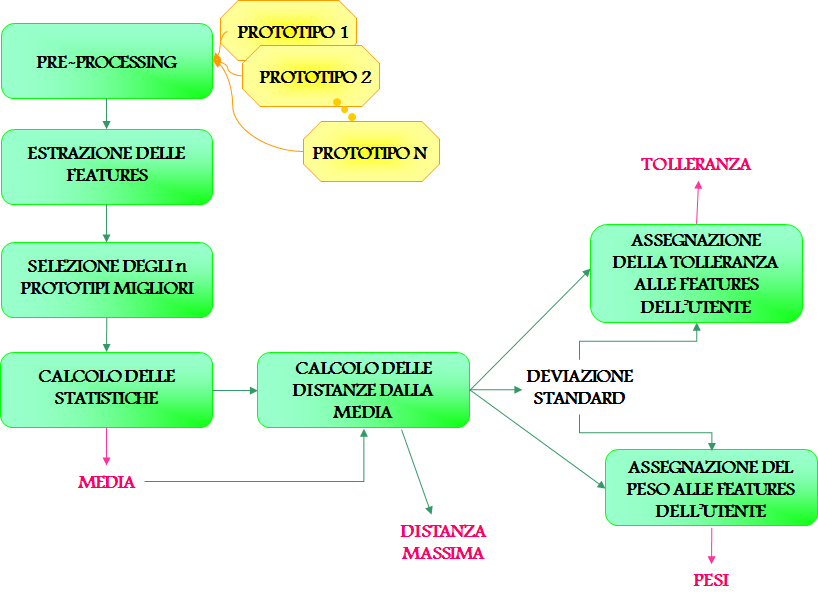
\includegraphics[scale=0.6]{../Logo&Header/trainingFirmatario.png}
\caption{Training per firmatario}Sorgente: Corvallis
\end{figure}

\subsubsection*{Fase di verifica}
\label{2.1.4.2}
Il processo di verifica prevede i seguenti step:
\begin{enumerate}
\item Estrazione delle \emph{feature} della firma di cui si vuole verificare l'autenticità, secondo la lista \emph{feature} e \emph{preprocessing} dell'utente che si vuole personificare;
\item Assegnazione dei voti;
\item Calcolo dei punteggi;
\item Calcolo della confidenza.
\end{enumerate}
\subsubsection*{Assegnazione dei voti}
\label{2.1.4.3}
Il valore di ogni \emph{feature} estratta dalla firma da verificare viene confrontato con la media corrispondente (presa dal \emph{feature centroid vector}). In base a quanto si scosta dalla media, ad ogni \emph{feature} viene assegnato un voto nell'intervallo [-1, 1].
\begin{itemize}
\item il voto è uguale a 1 (voto massimo possibile) quando la differenza tra il valore della \emph{feature} e la relativa media salvata è uguale a 0, ossia il valore della \emph{feature} è uguale alla media salvata.
\item il voto è uguale a -1 (voto minimo possibile) quando la differenza tra il valore della \emph{feature} e la relativa media salvata è maggiore o uguale a due volte la soglia.
\item altrimenti il voto viene assegnato secondo una funzione lineare:
\[Fvoto=\frac{Fthreshold-|FVal-Faverage|}{Fthreshold}\]
\end{itemize}
\subsubsection*{Calcolo dei punteggi}
\label{2.1.4.4}
Il core del sistema classifica le firme in base al punteggio che queste riescono a raggiungere. Il punteggio massimo raggiungibile è chiaramente la somma dei pesi delle \emph{feature}. Vediamo ora come si calcola il singolo punteggio che poi andrà a costituire parte del punteggio finale.
\[Fpunteggio=Fvoto * Fweight\]
Fvoto è il voto assegnato alla \emph{feature} F e Fweight è il peso della \emph{feature} F calcolato durante il training.
\subsubsection*{Calcolo della confidenza}
\label{2.1.4.5}
La decisione finale è data dal valore della confidenza. Se il valore della confidenza è maggiore di 50, la firma viene accettata altrimenti rifiutata. Il calcolo della confidenza è dato da:
\[Confidenza = \frac{0.5+\sum\limits_{i=1}^M FIpunteggio}{2*\sum\limits_{i=1}^M FIweight} * 100\]
M indica il numero di \emph{feature} prese in considerazione.\\\\
In figura 10 segue uno schema riassuntivo delle operazioni eseguite durante la fase di verifica.
\begin{figure}[H]
\centering
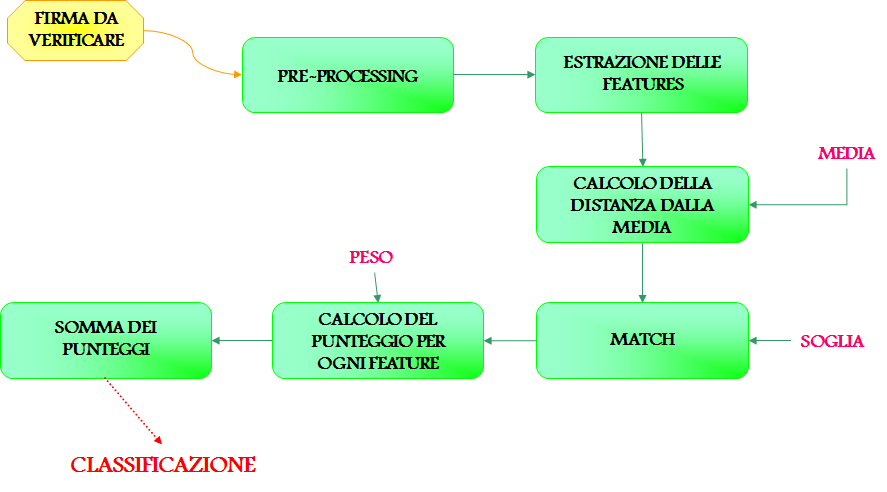
\includegraphics[scale=0.5]{../Logo&Header/verificaFirma.png}
\caption{Verifica firma}Sorgente: Corvallis
\end{figure}
\subsubsection*{Performance}
\label{2.1.4.6}
In tabella 1 vengono riportati i risultati di alcuni test.
\begin{table}[H]
  \label{tbl:excel-table}
  \centering
  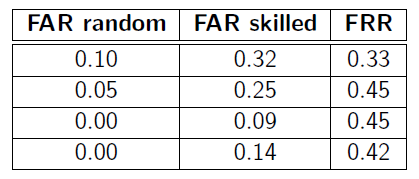
\includegraphics[scale=0.7]{../Logo&Header/overallResult.png}
  \caption{Risultati test prototipo preesistente}
\end{table}
\subsubsection*{Tecnologie impiegate}
\label{2.1.4.7}
Il prototipo è stato scritto in \emph{Java}, utilizzando l'\emph{Integrated development environment} (\emph{IDE}) \emph{Eclipse}. Le librerie utilizzate per l'elaborazione delle immagini sono \emph{ImageJ} e \emph{ImageMagick}. Il versionamento del codice è stato effettuato grazie a \emph{Content Versioning System} (\emph{CVS}).\\\\
\subsubsection*{ImageJ}
\label{2.1.4.8}
\emph{ImageJ} è un software \emph{open source}, prodotto dalla \emph{National Institute of Health} (\emph{NIH}) per la \emph{Macintosh}, sviluppato in linguaggio \emph{Java} esso nasce con l'obiettivo di emulare le funzionalità dei software per l'elaborazione delle immagini (\emph{image processing}). \'{E} un software portabile che può essere eseguito sia sotto forma di \emph{applet} (\emph{online}) che sotto forma di applicazione \emph{Java}. \emph{ImageJ} consente di visualizzare, modificare, analizzare, processare, salvare e stampare immagini a 8, 16 e 32 bit. Alcuni tra i formati supportati sono \emph{TIFF}, \emph{GIF}, \emph{JPEG}, \emph{BMP}, \emph{DICOM}, \emph{FTS} e \emph{RAW}. Inoltre permette di calcolare l'area e le statistiche sui valori dei pixel relativamente a delle regioni selezionate dall'utente (\emph{Region of interest}), di misurare distanze e angoli, di effettuare \emph{plotting} di grafici ed istogrammi. Infine supporta le più comuni trasformazioni geometriche come \emph{scaling}, rotazione... Le funzionalità di \emph{ImageJ} possono essere estese attraverso l'uso di \emph{plugin} scritti in \emph{Java}. I \emph{plugin} possono aggiungere supporto per nuovi formati file oppure possono filtrare e analizzare immagini.
\subsubsection*{ImageMagick}
\label{2.1.4.9}
\emph{ImageMagick} è una suite software per creare, editare, comporre o convertire immagini \emph{bitmap}. \'{E} in grado di leggere e scrivere oltre 100 formati tra cui ricordiamo \emph{DPX}, \emph{EXR}, \emph{GIF}, \emph{JPEG}, \emph{JPEG-2000}, \emph{PDF}, \emph{PhotoCD}, \emph{PNG}, \emph{Postscript}, \emph{SVG}, e \emph{TIFF}. \emph{ImageMagick} è in grado di ridimensionare, capovolgere, specchiare, ruotare, distorcere, tagliare e trasformare le immagini, regolare i colori delle immagini. Le funzionalità di \emph{ImageMagick} generalmente vengono utilizzate da riga di commando. Tuttavia sono state create interfacce per i linguaggi di programmazione più utilizzati in modo da permetterne l'utilizzo delle sue \emph{features} in programmi scritti in un linguaggio diverso.\\\\
La prossima sezione introduce il progetto di \emph{stage} a cui ho preso parte.

\subsection{Obiettivi}
\label{2.2}
L'obiettivo principale dello \emph{stage} è lo studio e l'implementazione di un nuovo classificatore di firme statiche, sempre nell'ambito dei classificatori \emph{Statistical-based}. Uno degli obiettivi secondari è testare approfonditamente il software preesistente per identificare le eventuali cause di un bug che rende la classificazione attuale dipendente dalla risoluzione del dispositivo di cattura. L'obiettivo ultimo è quello di valutare le performance del nuovo classificatore e di studiare una modalità di unione delle classificazioni dei due prototipi in modo da aumentare l'accuratezza globale del sistema di verifica delle firme statiche.
\subsection{Aspettative}
\label{2.3}
L'azienda si aspetta che l'obiettivo principale venga raggiunto.
\subsection{Vincoli}
\label{2.4}
Non sono stati imposti vincoli particolari per quanto riguarda lo svolgimento del progetto di \emph{stage}. I vincoli imposti sono:
\begin{itemize}
\item utilizzare il linguaggio \emph{Java} per l'implementazione del prototipo;
\item utilizzare \emph{Eclipse} come ambiente di sviluppo;
\item fornire documentazione adeguata sul prototipo implementato;
\item utilizzare le librerie \emph{ImageJ} e/o \emph{ImageMagick} per l'elaborazione delle immagini;
\item lo studio di nuovi metodi di classificazione deve avvenire sempre nell'ambito dei classificatori \emph{Statistical-based}.
\end{itemize}

\newpage

\section{Attività di stage}
\label{3.0}
Questo capitolo descrive le scelte operative effettuate, i problemi incontrati, gli effetti che questi ultimi hanno avuto sulla pianificazione stilata dal \emph{tutor} aziendale e le soluzioni adottate per raggiungere gli obiettivi del progetto di \emph{stage}. Per prima cosa introduco la pianificazione originale e il lavoro effettivamente svolto. Successivamente riporto i requisiti che il nuovo prototipo/classificatore dovrà soddisfare. In seguito illustro le decisioni prese in fase di progettazione. In conclusione spiego qualche particolare implementativo.
\subsection{Pianificazione}
\label{3.1}
Questa parte della relazione si prefigge di mostrare al lettore le discrepanze tra le attività pianificate e le attività effettivamente svolte.\\\\
Il piano di lavoro originale, redatto dal \emph{tutor} aziendale, prevedeva le seguenti macro attività suddivise settimanalmente come nel diagramma di \emph{Gantt} riportato in figura 11.
\begin{figure}[H]
\centering
\noindent\makebox[\textwidth]{%
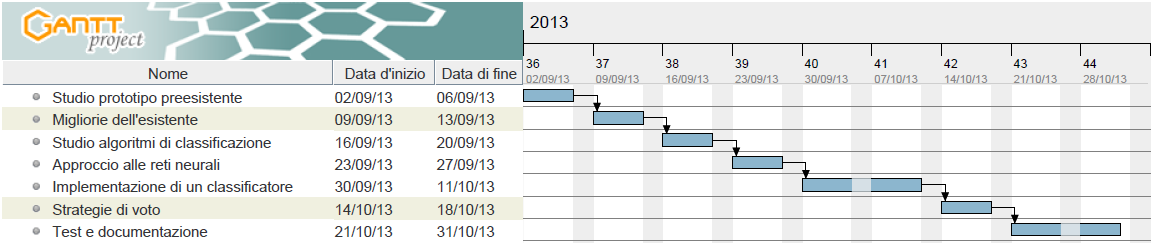
\includegraphics[scale=0.6]{../capitolo3img/pianificazioneIniziale.png}}
\caption{Diagramma di Gantt, Pianificazione iniziale}
\end{figure}
Lo \emph{stage} si è svolto nel periodo che va dal 02/09/2013 al 31/10/2013 per un totale di circa 330 ore.
Di seguito entro nel dettaglio di ogni settimana e descrivo il lavoro svolto.
\subsubsection{Settimane I-II}
\label{3.1.1}
%Le attività previste per le prime due settimane (dal piano di lavoro originale) vengono riportate nel diagramma di \emph{Gantt} in figura 12.
%\begin{figure}[H]
%\centering
%\noindent\makebox[\textwidth]{%
%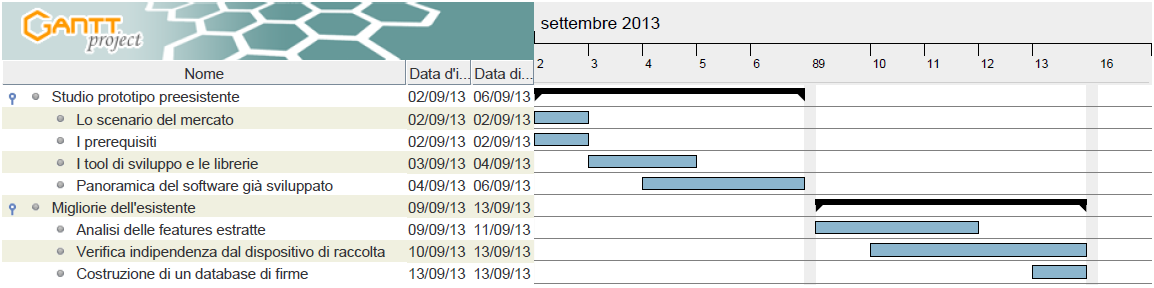
\includegraphics[scale=0.6]{../capitolo3img/settIeII.png}}
%\caption{Diagramma di Gantt, Settimane I-II}
%\end{figure}
La prima settimana prevedeva attività di studio del dominio applicativo in cui si colloca il progetto di \emph{stage}.\\
Vediamo una breve descrizione di ciascuna attività effettuata.
\begin{itemize}
\item lo scenario di mercato: il \emph{tutor} aziendale mi ha spiegato che la normativa italiana relativa allo scambio di immagini degli assegni bancari sta per essere aggiornata, in quanto a questi sarà concesso lo scambio di immagini di assegni bancari, e le conseguenze che ne scaturiscono;
\item i prerequisiti: le condizioni iniziali sono individuate dalla capacità di un software di estrarre immagini firma da assegni bancari, di classificare le suddette firme in relazione a una base di conoscenza precedentemente acquisita, di essere affidabile;
\item i \emph{tool} di sviluppo e le librerie: durante questa attività ho familiarizzato con le tecnologie impiegate nello sviluppo del prototipo sviluppato precedentemente;
\item panoramica del software preesistente: nel corso di questa attività ho compreso sommariamente i meccanismi adottati per la classificazione delle immagini firma sia a livello interattivo (utilizzo del software) che a livello di codice implementato.
\end{itemize}
La seconda settimana prevedeva un'analisi più accurata del software sviluppato precedentemente allo scopo di identificare la causa di un'eventuale bug che rende la classificazione dipendente dalla risoluzione del dispositivo di raccolta immagini (scanner o tavoletta).\\\\
Data la mia esperienza nulla nell'elaborazione delle immagini, ho ritenuto opportuno effettuare test utilizzando la tecnica \emph{Walktrough} e non la tecnica \emph{Inspection}. Ho analizzato la maggior parte degli algoritmi di \emph{feature extraction} per individuare un qualche collegamento implicito con la risoluzione dell'immagine processata.\\Le mie ricerche non sono riuscite a dimostrare se il software è dipendente o meno dalla risoluzione del dispositivo di acquisizione immagini. Nonostante ciò potrebbero aver individuato leggerissime migliorie da apportare al calcolo del punteggio (paragrafo \ref{2.1.4.4}) di quelle \emph{feature} che assumono valori discreti, poiché per queste, in fase di test, il voto massimo non è raggiungibile e di conseguenza subiscono una penalità.
\subsubsection*{Considerazioni sulle prime due settimane}
\label{3.1.1.1}
Le attività previste per le prime due settimane sono state effettuate come pianificato e sono state di fondamentale importanza per l'Analisi dei Requisiti. Tuttavia la seconda settimana non ha portato i risultati sperati.
\subsubsection{Settimane III-IV}
\label{3.1.2}
%Le attività previste per la terza e la quarta settimana (dal piano di lavoro originale) vengono riportate nel diagramma di \emph{Gantt} in figura 13.
%\begin{figure}[H]
%\centering
%\noindent\makebox[\textwidth]{%
%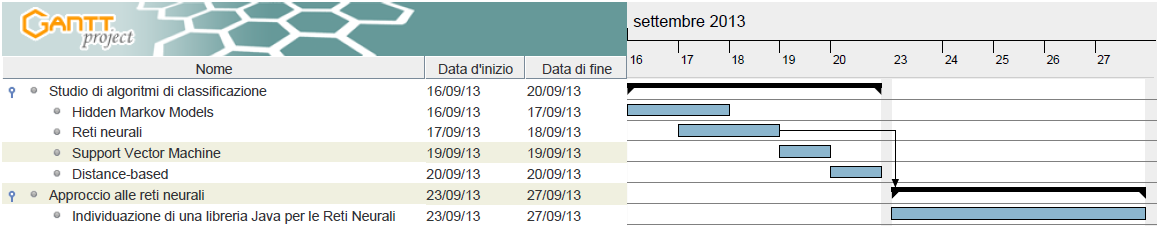
\includegraphics[scale=0.6]{../capitolo3img/settIIIeIV.png}}
%\caption{Diagramma di Gantt, Settimane III-IV}
%\end{figure}
La terza settimana prevedeva lo studio critico, attraverso materiale \emph{online} di natura scientifica, dei meccanismi di classificazione di tipo \emph{Statistical-based} più diffusi in modo da stimare in modo opportuno le potenzialità di ciascuno.\\\\
Tuttavia l'attività effettivamente svolta è stata lo studio dei \emph{Hidden Markov Model} utilizzati nella classificazione di firme statiche. Poiché, già dai primi articoli analizzati \cite{3}\cite{5}\cite{6}, si evinceva che i \emph{Hidden Markov Models} avrebbero potuto portare dei buoni risultati in termini di \emph{accuracy}, il \emph{tutor} aziendale e io abbiamo deciso di investire le ore (della settimana) rimaste nello studio approfondito di tale modello e di non attenerci al piano di lavoro originale. Inoltre sono stato assente gli ultimi due giorni lavorativi della settimana.\\\\
La quarta settimana prevedeva l'approccio alle reti neurali e l'individuazione di una libreria \emph{Java} che ne implementi le meccaniche.\\\\Chiaramente, vista la scelta effettuata durante la terza settimana, questa attività non poteva essere messa in atto. Di conseguenza le operazioni compiute hanno avuto lo scopo di individuare una libreria \emph{Java} che implementa la dinamica dei \emph{Hidden Markov Model}. Dopo aver individuato una libreria ho abbozzato un prototipo usa e getta.
\subsubsection*{Considerazioni sulla terza e quarta settimana}
Le attività previste per questo periodo non hanno osservato il piano di lavoro originale. La progettazione iniziale si basa sullo studio effettuato in queste due settimane.
\label{3.1.2.1}
\subsubsection{Settimane V-VI}
\label{3.1.3}
Per la quinta e la sesta settimana era prevista l'implementazione di un classificatore in modo prototipale, ma che sarebbe dovuto essere sufficiente a dimostrare la validità del metodo di classificazione scelto.\\\\
Le attività compiute durante la quinta e la sesta settimana sono riportate nel diagramma di \emph{Gantt} in figura 14.
\begin{figure}[H]
\centering
\noindent\makebox[\textwidth]{%
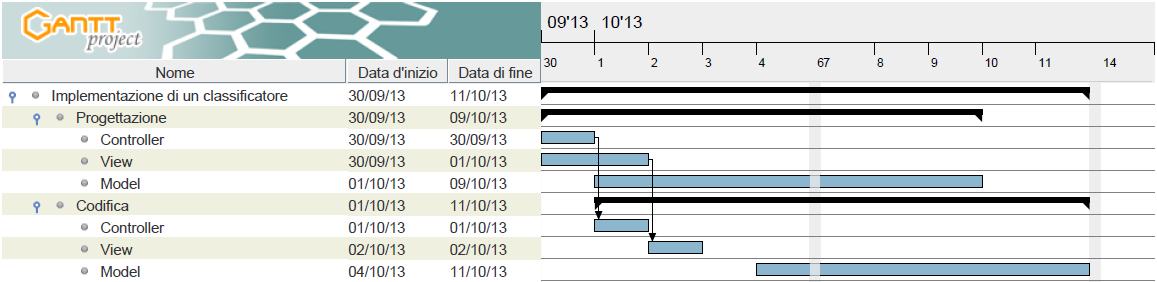
\includegraphics[scale=0.6]{../capitolo3img/settVeVI.png}}
\caption{Diagramma di Gantt, attività svolte settimane V-VI}
\end{figure}

Come si può notare nel diagramma di \emph{Gantt} questa fase è stata suddivisa in due sotto-fasi che si sovrappongono:
\begin{itemize}
\item Progettazione;
\item Codifica;
\end{itemize}
Le attività di progettazione dei componenti \emph{Controller} e \emph{View} del pattern architetturale \emph{MVC} (paragrafo \ref{3.3.1}) hanno richiesto relativamente poco tempo. Questo è dovuto al fatto che è stato possibile riutilizzare parti di architettura del software preesistente. Di conseguenza l'operazione di codifica dei suddetti componenti è stata più un'integrazione che una vera e propria implementazione.\\\\
Purtroppo la progettazione del componente \emph{Model}, dato l'ambito esplorativo in cui si colloca il progetto di \emph{stage}, ha richiesto molto tempo. Questo è dovuto principalmente al ritardo con cui si sono presentati i punti più sensibili relativi all'utilizzo dei \emph{Hidden Markov Models}. Questi sono emersi durante la codifica iniziale e vengono esposti in modo approfondito nella sezione Progettazione (\ref{3.3}).


\subsubsection*{Considerazioni sulla quinta e sesta settimana}
\label{3.1.3.1}
Le attività svolte in questo periodo hanno portato a una più estesa comprensione dei \emph{Hidden Markov Model}. Tuttavia permangono dei problemi con l'algoritmo che permette di addestrare un \emph{Hidden Markov Model} e di conseguenza il prototipo in questo stadio non è stabile.
\subsubsection{Settimane VII-IX}
\label{3.1.4}
Le attività previste per l'ultima parte del progetto comprendevano lo studio di una strategia di classificazione unita tra il prototipo realizzato durante lo \emph{stage} e il software preesistente, i test e la documentazione.\\\\
Le attività effettivamente svolte nelle ultime due settimane vengono riportate nel diagramma di \emph{Gantt} in figura 15.
\begin{figure}[H]
\centering
\noindent\makebox[\textwidth]{%
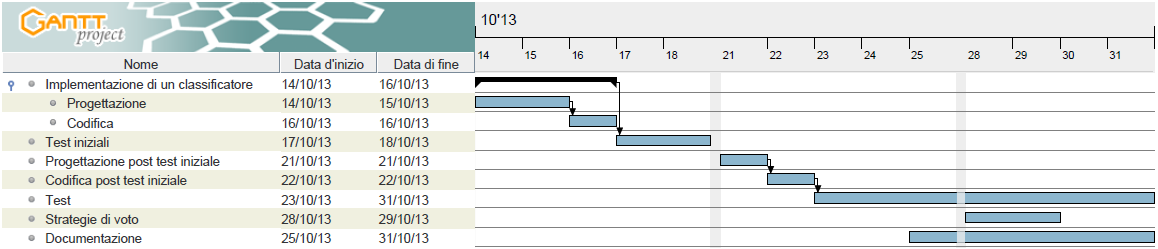
\includegraphics[scale=0.6]{../capitolo3img/settVIIeVIII.png}}
\caption{Diagramma di Gantt, attività svolte settimane VII-IX}
\end{figure}
Come si può notare nel diagramma di \emph{Gantt} relativo a questo periodo, nei primi giorni della settima settimana sono riuscito a finire l'implementazione del prototipo. Tuttavia durante i test iniziali ci siamo accorti di un altro problema che avevamo ignorato: alcuni modelli addestrati sono caduti nell'eccessivo adattamento e la loro capacità di categorizzare firme non visionate è stata compromessa.\\\\
Durante l'inizio dell'ottava settimana ho studiato come arginare il problema dell'eccessivo adattamento e ne ho implementato una soluzione basata sulla cross-validazione. Test, successive correzioni di bug e documentazione si sono susseguite fino alla fine dello \emph{stage}.\\\\
All'inizio dell'ultima settimana ho studiato e implementato un metodo di classificazione comune che si basa sulle decisioni del prototipo preesistente al progetto di \emph{stage} e del prototipo sviluppato durante.
\subsubsection*{Considerazioni sul periodo finale}
\label{3.1.4.1}
I test sono utili solo se identificano comportamenti non prescritti.
\subsection{Analisi}
\label{3.2}

Il progetto di \emph{stage} prevedeva l'implementazione di un nuovo classificatore di firme. In seguito allo studio del dominio applicativo effettuato durante le prime due settimane di \emph{stage} e alle spiegazioni del \emph{tutor} aziendale sono riuscito ad individuare i requisiti del prototipo richiesto.\\\\
Poiché si tratta di un prototipo, esso non sarà collocato nell'ambito applicativo di competenza (applicazione per istituti bancari) e soprattutto non sarà indipendente dal input umano. Dovrà essere un'applicazione locale in grado di addestrare la sua base di conoscenza e grazie all'addestramento dovrà essere in grado di classificare immagini firma. L'analisi dei requisiti è stata effettuata seguendo questi cardini semplicistici.\\\\
Di seguito vengono riportati i casi d'uso principali individuati.
\subsubsection{Casi d'uso}
\label{3.2.1}
I casi d'uso (\emph{use case}) sono tecniche per individuare i requisiti funzionali. Essi descrivono interazioni del sistema e degli attori esterni al sistema e come il sistema deve essere utilizzato \cite{7}.
L'attore principale è uno solo: utente che configura e avvia il prototipo a piacimento.
\subsubsection*{UC1 Caso d'uso generale}
\label{3.2.1.1}
\textbf{Scopo e descrizione}: un utente deve poter selezionare un database di firmatari e rispettive firme. Una volta selezionato il database, deve essere possibile effettuare il training impostando il numero di firme da utilizzare e i preprocessing. Ultimato il training deve essere possibile testare l'accuratezza del sistema classificando le firme restanti nel database.\\\\
\textbf{Precondizione}: il sistema si trova nello stato iniziale.\\\\
\textbf{Postcondizione}: il sistema restituisce e salva su file i risultati relativi alla classificazione effettuata.\\\\
\textbf{Scenario principale}:
\begin{itemize}
\item l'utente seleziona il database di firme su cui lavorare;
\item l'utente configura i parametri disponibili;
\item l'utente avvia il training;
\item l'utente avvia il testing.
\end{itemize}

\subsubsection*{UC1.3 Avvia training}
\label{3.2.1.2}
\textbf{Scopo e descrizione}: un utente deve poter avviare il training su un database con impostazioni a piacimento.\\\\
\textbf{Precondizione}: il sistema conosce il database selezionato dall'utente e i parametri che quest'ultimo ha impostato precedentemente.\\\\
\textbf{Postcondizione}: il sistema addestra la sua base di conoscenza secondo la configurazione dell'utente e la salva su file.\\\\
\textbf{Scenario principale}:
\begin{itemize}
\item l'utente avvia il training.
\end{itemize}
\subsubsection*{UC1.4 Avvia testing}
\label{3.2.1.3}
\textbf{Scopo e descrizione}: un utente deve poter avviare il testing sulle firme (di un database) non visionate in fase di training.\\\\
\textbf{Precondizione}: il sistema conosce il database selezionato dall'utente e la base di conoscenza del database è stata addestrata in precedenza.\\\\
\textbf{Postcondizione}: il sistema restituisce i risultati della classificazione e li salva su file.\\\\
\textbf{Scenario principale}:
\begin{itemize}
\item l'utente avvia il testing.
\end{itemize}
Il diagramma \emph{use case} che descrive le macro funzionalità del prototipo segue in figura 16.
\begin{figure}[H]
\centering
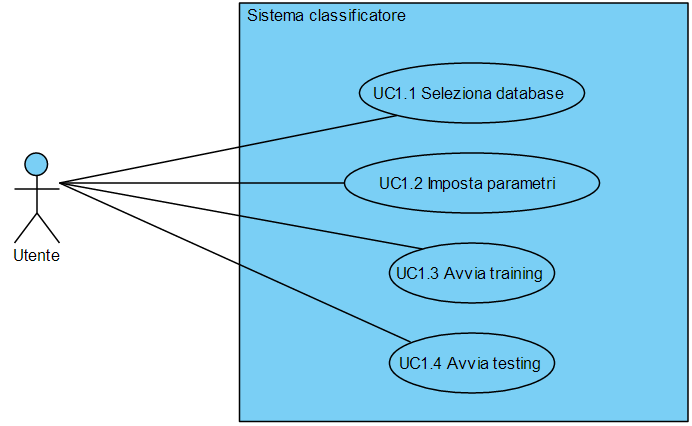
\includegraphics[scale=0.7]{../capitolo3img/uc1.png}
\caption{Diagramma use case, UC1 caso d'uso generale}
\end{figure}


\subsubsection{Requisiti}
\label{3.2.2}
La classificazione dei requisiti sarà conforme al seguente formalismo:
\[R\{TIPO\}\{IMPEGNO\}\{GERARCHIA\}\]
dove:
\begin{itemize}
\item\textbf{TIPO} può essere:
	\begin{itemize}
	\item\emph{F}, indica un requisito funzionale
	\item\emph{Q}, indica un requisito di qualità
	\item\emph{V}, indica un requisito di vincolo
	\end{itemize}
\item\textbf{IMPEGNO} può essere:
	\begin{itemize}
	\item\emph{O}, indica un requisito obbligatorio, ossia il soddisfacimento di questo vincolo è necessario per la realizzazione del prodotto finale
	\item\emph{D}, indica un requisito desiderabile, ossia un requisito auspicabile per un prodotto di qualità
	\end{itemize}
\item\textbf{GERARCHIA}: i requisiti sono organizzati gerarchicamente secondo una struttura ad albero. Un requisito (padre) può essere complesso al punto di dover essere suddiviso in requisiti minori (figli). X.Y individua un requisito Y figlio di un requisito X.
\end{itemize}

I requisiti determinati a partire dall'obiettivo principale del progetto di \emph{stage} vengono riportati in tabella 2.
\begin{longtable}{|c|p{9cm}|c|}
\caption{Requisiti}
\label{tab:Requisiti} \\
\toprule
\multicolumn{1}{|c}{\textbf{\underline{Requisito}}} & \multicolumn{1}{|p{9cm}}{\textbf{Descrizione}} & \multicolumn{1}{|c|}{\textbf{Caso d'uso}}\\
\midrule
\endfirsthead
\multicolumn{2}{l}{\footnotesize\itshape\tablename~\thetable: continua dalla pagina precedente} \\
\toprule
\multicolumn{1}{|c}{\textbf{Requisito}} & \multicolumn{1}{|p{9cm}}{\textbf{Descrizione}}   & \multicolumn{1}{|c|}{\textbf{Caso d'uso}}\\
\midrule
\endhead
\midrule
\multicolumn{2}{r}{\footnotesize\itshape\tablename~\thetable: continua nella prossima pagina} \\
\endfoot
\bottomrule
\multicolumn{2}{r}{\footnotesize\itshape\tablename~\thetable: si conclude dalla pagina precedente} \\
\endlastfoot



\midrule
RFO1
& Il sistema deve essere in grado di classificare in modo corretto immagini di firma autografa in seguito a una fase di training eseguita conformemente alle impostazioni utente, su un database selezionato precedentemente.
& UC1
\\
\midrule
RFO1.1
& Il sistema deve permettere all'utente di selezionare un database di firmatari con le rispettive firme.
& UC1.1
\\
\midrule
RFO1.2
& Il sistema deve poter caricare in memoria il file di configurazione dei parametri impostato dall'utente.
& UC1.2
\\
\midrule
RFO1.3
&  Il sistema deve permettere all'utente di effettuare il training su un database selezionato precedentemente.
& UC1.3
\\
\midrule
RFO1.3.1
& Il sistema deve essere in grado di elaborare il template/firma media di un firmatario a partire da N firme genuine del sottoscrittore.
& UC1.3
\\
\midrule
RFO1.3.2
& Il sistema deve essere in grado di salvare il template su file.
& UC1.3
\\
\midrule
RFO1.4
& Il sistema deve essere in grado di classificare correttamente firme che non ha mai visionato.
& UC1.4
\\
\midrule
RFO1.4.1
& Il sistema deve essere in grado di caricare in memoria il template/firma media del sottoscrittore la cui firma si sta testando.
& UC1.4
\\
\midrule
RFO1.4.2
& Il sistema deve essere in grado di confrontare la firma sotto test con il template del sottoscrittore.
& UC1.4
\\
\midrule
RFO1.4.3
& Il sistema deve essere in grado di prendere una decisione sul risultato del confronto e quindi accettare o rifiutare la firma sotto test.
& UC1.4
\\
\midrule
RFO1.4.4
& Il sistema deve essere in grado di riportare a video e salvare su file il risultato della classificazione.
& UC1.4
\\
\midrule
RFV2
& Il core del sistema deve essere un classificatore di tipo \emph{Statistical-based}.
&
\\
\midrule
RFQ3
& Il sistema deve garantire un'\emph{accuracy} media del 80\%.
& 
\end{longtable}
Il test sul output dell'attività di analisi ha compreso test di natura statica sui requisiti. In particolare ho verificato la loro atomicità, chiarezza di esposizione e completezza.\\\\
Il modello di ciclo di vita del software selezionato è quello incrementale. Fra i vantaggi dei modelli incrementali ricordiamo\cite{7}:
\begin{itemize}
\item si può produrre valore ad ogni incremento;
\item ogni incremento riduce il rischio di fallimento;
\item le funzionalità essenziali sono sviluppate nei primi incrementi.
\end{itemize}
Questa scelta è stata effettuata poiché i requisiti principali sono identificati e fissati in modo completo e perché l'architettura del sistema era già stata osservata nel prototipo preesistente durante le prime due settimane di \emph{stage}.\\\\
\subsection{Progettazione}
\label{3.3}
Questa parte della relazione vuole mostrare al lettore le scelte progettuali effettuate relative all'architettura e alle tecnologie da impiegare per soddisfare i requisiti individuati in fase di analisi.
\subsubsection{Architettura}
\label{3.3.1}
L'architettura è l'output della fase di progettazione, essa ha l'obiettivo di rendere l'attività di programmazione il più vincolata possibile senza lasciare spazio all'interpretazione.\\\\
Poiché il software preesistente utilizza il pattern architetturale \emph{Model View Controller} ho deciso di adoperarlo anche io. I vantaggi principali di un'architettura \emph{MVC} si possono riassumere nei seguenti punti:
\begin{itemize}
\item consente di tenere una netta separazione tra le componenti di stato (\emph{Model}), i componenti mostrati sullo schermo (\emph{View}) e
il loro comportamento in relazione agli eventi (\emph{Controller});
\item manutenibilità del software;
\item modularità;
\item leggibilità.
\end{itemize}
In figura 17 è possibile visionare il pattern MVC.
\begin{figure}[H]
\centering
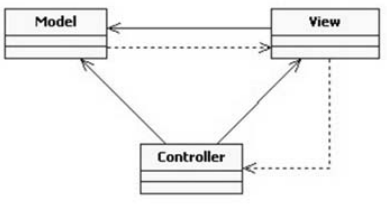
\includegraphics[scale=0.7]{../capitolo3img/mvc.png}
\caption{Pattern MVC}
\end{figure}
\subsubsection{Hidden Markov Models}
\label{3.3.2}
Questa sezione effettua una panoramica sui \emph{Hidden Markov Models}, spiegandone le dinamiche, la modellazione delle firme, i problemi incontrati e le soluzioni adottate per superarle.\\\\
Segue un'introduzione ai modelli di Markov.
\subsubsection*{Processo di Markov}
\label{3.3.2.1}
Un processo (sistema) di Markov è contraddistinto dalle seguenti affermazioni:
\begin{itemize}
\item ha N stati distinti : S\ped{1}, S\ped{2}, ..., S\ped{N};
\item è caratterizzato da passi discreti, t=1, t=2, ...
\item la probabilità di partire da un determinato stato è data dalla \gls{matrice stocastica}: 
\[ \Pi =\{\pi\ped{i}\}: \pi\ped{i}=P(q\ped{1} = s\ped{i})\ con\ 1\le i\le N,\  \pi\ped{i}\ge 0\  e\  \sum\limits_{i=1}^N \pi\ped{i} = 1 \]
\item al t-esimo istante il processo si trova esattamente in uno degli stati a disposizione, indicato dalla variabile q\ped{t}:
\[ q\ped{t} \in \{S\ped{1}, S\ped{2}, ..., S\ped{N}\}\]
\item ad ogni iterazione, lo stato successivo viene scelto con una determinata probabilità. Tale probabilità è solo ed esclusivamente dipendente dallo stato precedente, e non dalla sequenza di stati che lo ha preceduto (\emph{memoryless}). Questa dichiarazione riassume la \emph{proprietà di Markov}:
\[ P(q\ped{t+1}=s\ped{j}\ |\ q\ped{t}=s\ped{i},\ q\ped{t-1}=s\ped{k},\ ...,\ q\ped{1}=s\ped{1})\ =\ P(q\ped{t+1}=s\ped{j}\ |\ q\ped{t}=s\ped{i})\]
\item le probabilità di transizione tra stati (invarianti nel tempo) sono descritte dalla matrice stocastica:
\[ A=\{a\ped{ij}\}\ :\ a\ped{ij}=P(q\ped{t+1}=s\ped{j}\ |\ q\ped{t}=s\ped{i})\]
\end{itemize}
\subsubsection*{Modello di Markov}
\label{3.3.2.2}
Date le caratteristiche del processo di Markov descritte nella sezione precedente un modello di Markov si può riassumere con:
\[\lambda=(A,\ \pi)\]
Le operazioni interessanti che si possono effettuare sui modelli di Markov sono:
\begin{itemize}
\item addestramento o training (si costruiscono gli elementi costituenti del modello);
\item interrogazioni sul modello per esempio calcolare la probabilità di una sequenza di stati, dato il modello.
\end{itemize}
I modelli di Markov modellano processi Markoviani in cui gli stati sono espliciti e osservabili: c'è una corrispondenza biunivoca tra le osservazioni e i stati emittenti. Purtroppo nella realtà esistono modelli i cui stati non sono espliciti, essi sono identificabili unicamente tramite le osservazioni, in maniera probabilistica. All'osservatore è accessibile soltanto una sequenza di simboli in base alla quale egli può inferire soltanto la probabilità degli stati corrispondenti. Questi modelli vengono denominati modelli di Markov a stati nascosti.
\subsubsection*{Hidden Markov Model}
\label{3.3.2.3}
Il modello di Markov a stati nascosti può essere inteso come un' estensione del modello di Markov che si distingue per la non osservabilità dei suoi stati. Esso si compone di:
\begin{itemize}
\item un insieme S=\{S\ped{1},S\ped{2},...,S\ped{N}\} di stati nascosti;
\item una matrice di transizione tra stati nascosti:
\[ A=\{a\ped{ij}\}\ :\ a\ped{ij}=P(q\ped{t+1}=s\ped{j}\ |\ q\ped{t}=s\ped{i})\]
\item una matrice di probabilità di partire da uno stato iniziale nascosto:
\[ \Pi =\{\pi\ped{i}\}: \pi\ped{i}=P(q\ped{1} = s\ped{i})\ con\ 1\le i\le N,\  \pi\ped{i}\ge 0\  e\  \sum\limits_{i=1}^N \pi\ped{i} = 1 \]
\item un insieme V=\{V\ped{1},V\ped{2},...,V\ped{M}\} di simboli di osservazione;
\item al t-esimo istante il processo emette uno fra i simboli a disposizione, indicato dalla variabile o\ped{t}:
\[o\ped{t} \in\{V\ped{1},V\ped{2},...,V\ped{M}\}\]
\item una matrice stocastica con le probabilità di emissione, indica la probabilità di osservare il simbolo V\ped{k} quando il sistema si trova nello stato S\ped{j}:
\[ B=\{b\ped{j}(k)\}\ : b\ped{j}(k)=P(o\ped{t}=k\ |\ q\ped{t}=j)\]
\end{itemize}
In generale un \emph{HMM} si indica con la tripla
\[ \lambda=(A,\ B,\ \pi)\]
\subsubsection*{Tipi di \emph{Hidden Markov Models}}
\label{3.3.2.4}
I Hidden Markov Models possono venire classificati in base alla topologia degli stati o in base a cosa rappresentano i simboli.\\\\
Topologie:
\begin{itemize}
\item modelli ergodici, se è possibile andare da ogni stato i ad ogni stato j, non necessariamente in un solo step;
\item modelli \emph{Left to Right} o \emph{Bakis}, se la matrice delle probabilità di transizione è una matrice triangolare superiore (l'indice degli stati non decresce col tempo). Questa topologia viene adottata per la modellazione delle firme perché si assume che la scrittura latina vada da sinistra verso destra.
\end{itemize}
In figura 18 è possibile visualizzare le due topologie.
\begin{figure}[H]
\centering
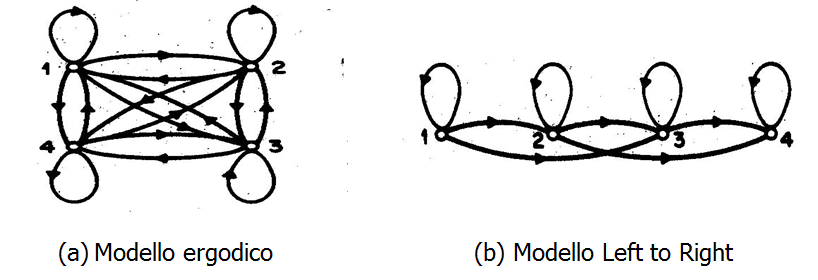
\includegraphics[scale=0.7]{../capitolo3img/topologie.png}
\caption{Topologie HMM}
\end{figure}
Nel \emph{discrete HMM} i simboli sono discreti, mentre nel \emph{continuous HMM} i simboli sono vettori. Nel primo caso, B\ped{j} è una matrice, mentre nel secondo caso B\ped{j} è una \emph{mixture of gaussian probalility density functions}.

\subsubsection*{I tre problemi dei \emph{Hidden Markov Models}\cite{8}}
\label{3.3.2.5}
\begin{enumerate}
\item\textbf{\emph{Evaluation}}, dato un modello di Markov a stati nascosti $\lambda$ e una sequenza d'osservazione O, trovare la probabilità che la sequenza O possa venire generata dal modello $\lambda$ : P(O$|\lambda$);
\item\textbf{\emph{Decoding}}, dato un HMM $\lambda$ e una sequenza O, trovare la sequenza di stati $\pi$\ped{i} più probabile (\emph{most probable path}) che massimizza P(O, $\pi$\ped{i}$|\lambda$);
\item\textbf{\emph{Learning}}, dato un modello $\lambda$ con transizioni ed emissioni non note e una sequenza d'osservazione O trovare le matrici A e B tali che P(O$|\lambda$) è massimo. In altre parole vorremmo usare la sequenza d'osservazione per addestrare un \emph{HMM}. Questo è il problema più difficoltoso perchè non esiste un metodo analitico per la sua soluzione.
\end{enumerate}
\subsubsection*{Soluzioni ai problemi individuati\cite{8}}
\label{3.3.2.6}
Poiché in generale i 3 problemi sono computazionalmente intrattabili, delle soluzioni basate sulla \gls{programmazione dinamica} sono state adottate.
\begin{enumerate}
\item\textbf{\emph{Forward algorithm}}, poiché sommare le probabilità di tutti i possibili modi in cui si può generare la sequenza O coinvolge un numero esponenziale di cammini $\pi$ si definisce probabilità \emph{forward}:
\[ f\ped{t}(i)=P(O\ped{1}...O\ped{t},\ \pi\ped{t}=i)\]
può essere derivata ricorsivamente:
\begin{itemize}
\item caso base
\[f\ped{1}(i)=P(\pi\ped{1=i}*b\ped{i}(O\ped{1})\ con\ 1\le\ i\le\ k\]
\item passo induttivo
\[f\ped{t+1}(j)=[\ \sum\limits_{i=1}^k f\ped{t}(i)*a(i,j)\ ]*b\ped{j}(O\ped{t+1})\]
\end{itemize}
\item\textbf{\emph{Viterbi's algorithm}}, per una descrizione si rimanda al documento\cite{8};
\item\textbf{\emph{Baum-Welch algorithm}}, algoritmo iterativo di \emph{expectation-maximization} basato sul \emph{forward-backward algorithm} e \emph{Viterbi's algorithm}. Può convergere a massimi locali, dipende dai valori assunti dalle matrici iniziali.
\end{enumerate}
I campi in cui vengono applicati i \emph{HMM} sono molteplici. Di seguito riportiamo alcuni di questi:
\begin{itemize}
\item riconoscimento della parola;
\item sintesi vocale;
\item riconoscimento texture;
\item riconoscimento movimento del corpo;
\item riconoscimento della grafia.
\end{itemize}
\subsubsection*{Modello HMM che descrive le firme di un sottoscrittore}
\label{3.3.2.7}
Vediamo ora come ho inizializzato e addestrato un modello di Markov a stati nascosti che descrive le firme di un sottoscrittore.\\\\
La scelta del numero di stati nascosti che si assume siano presenti è un punto fondamentale. In letteratura hanno utilizzato due diversi approcci:
\begin{itemize}
\item in \cite{3} suggeriscono di non impostare il numero di stati nascosti a priori ma di calcolarlo in base alla larghezza della firma;
\item in \cite{5} decidono a priori il numero di stati nascosti e lo impostano a 4.
\end{itemize}
Per semplicità ho scelto la seconda strada.\\\\
Ricordiamo che un \emph{HMM} è caratterizzato dalla tripla $\lambda$=(A,B,$\pi$). Come abbiamo accennato in precedenza la topologia che meglio descrive le firme latine (scritte da sinistra verso destra) è la \emph{Left to Right}. L'uso di questa topologia rende l'inizializzazione delle matrici A e $\pi$ banale. Come indicato nel documento \cite{3} ho aggiunto un ulteriore vincolo sulla matrice delle probabilità di transizione (A): i salti di stato non sono ammessi.\\\\
Vediamo le matrici A e $\pi$ risultanti:
\[A=\left| \begin{array}{cccc}
0.95&0.05&0&0 \\
0&0.95&0.05&0 \\
0&0&0.95&0.05 \\
0&0&0&1.0 \end{array} \right|\]
\[\pi=\left| \begin{array}{cccc}
1.0&0&0&0 \end{array} \right|\]
Per quanto riguarda la matrice delle probabilità di emissione ho scelto di utilizzare i \emph{discrete HMM}.\\\\
Vediamo ora i passi progettati per l'inizializzazione della matrice B:
\begin{itemize}
\item \emph{feature extraction}, poiché servono delle \emph{features} ho deciso di testare la \emph{feature axial slant} (come in \cite{3}) e la \emph{feature Discrete Cosine Transform (DCT)} (come in \cite{5}).
\item tipi di \emph{preprocessings}, ho deciso di testare la segmentazione a griglia (come in \cite{3}) per la \emph{feature axial slant} e la segmentazione basata sul centro di gravità per la \emph{feature DCT}\cite{5}. Entrambe le segmentazioni dividono l'immagine firma in 64 celle.
\item la fase di \emph{feature extraction} restituisce 64 valori (un valore per cella). Questi costituiscono 4 vettori d'osservazione per firma.
\item i punti sopra descritti vanno effettuati per tutte le firme che si intendono utilizzare nella fase di training
\item i vettori ottenuti vengono dati in pasto al metodo \emph{KMeansLearner} della libreria \emph{JScience}, il quale effettua il \emph{clustering} e inizializza la matrice B.
\end{itemize}
In figura 19 è disponibile una figura che riporta i passi eseguiti per individuare i  vettori d'osservazione.
\begin{figure}[H]
\centering
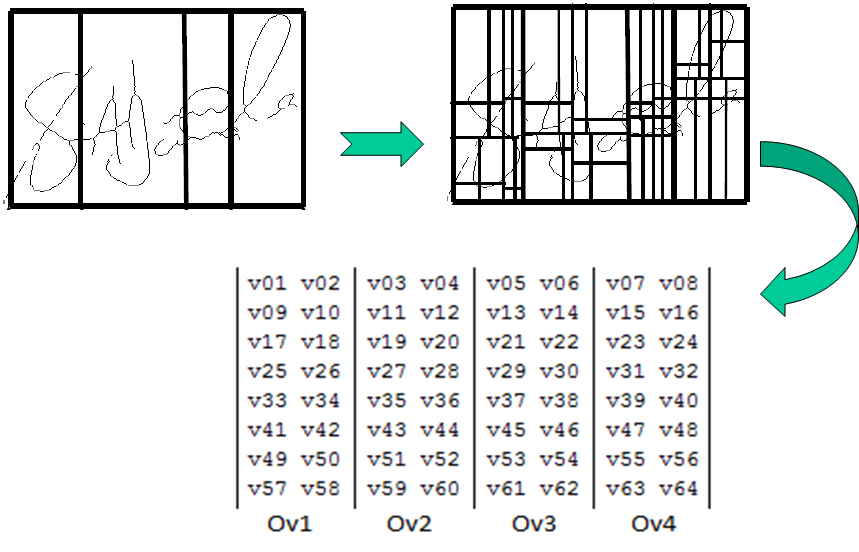
\includegraphics[scale=0.6]{../capitolo3img/matriceB.png}
\caption{Dalla firma ai vettori d'osservazione}
\end{figure}
Per quanto riguarda l'addestramento del modello, basta applicare l'algoritmo di \emph{Baum-Welch}.

\subsubsection{Tecnologie utilizzate}
\label{3.3.3}
Di seguito vengono elencate le tecnologie utilizzate per lo sviluppo del prototipo.

\subsubsection*{\emph{Java}}
\label{3.3.3.1}
Ho utilizzato il linguaggio \emph{Java} come richiesto dall'azienda. Fra i vantaggi che il linguaggio \emph{Java} offre ricordiamo:
\begin{itemize}
\item compatibilità multipiattaforma (grazie alla \emph{Virtual Machine});
\item velocità di sviluppo;
\item grande disponibilità di librerie;
\item alta integrazione con il web;
\item incoraggia il riutilizzo del codice.
\end{itemize}

\subsubsection*{\emph{Eclipse}}
\label{3.3.3.2}
Ho utilizzato l'ambiente di sviluppo \emph{Eclipse} come richiesto dall'azienda. I vantaggi di questo vincolo si possono riassumere in:
\begin{itemize}
\item navigazione intelligente del codice;
\item \emph{code completion} integrata;
\item compilazione al volo.
\end{itemize}

\subsubsection*{\emph{ImageJ}}
\label{3.3.3.3}
Per l'elaborazione delle immagini ho utilizzato la libreria \emph{ImageJ} perché è di facile comprensione e non richiede uno step in più per il \emph{preprocessing} delle immagini, quale l'utilizzo del terminale.

\subsubsection*{Persistenza dei dati}
\label{3.3.3.4}
Le immagini firma sono salvate in formato \emph{PNG} all'interno di cartelle individuate dal nome del sottoscrittore dentro una cartella (database) contenente i sottoscrittori. A ciascun sottoscrittore corrisponde uno o più file di \emph{properties} (a seconda dello stato del database: training effettuato o meno) che riassumono i \emph{preprocessings}, le \emph{features} estratte, l'eventuale \emph{template}/modello di firma calcolato durante la fase di training.
\subsubsection*{Librerie \emph{Java} che implementano i \emph{HMM}}
\label{3.3.3.5}
In seguito alla decisione di adoperare i \emph{Hidden Markov Models} per la classificazione di firme statiche, abbiamo effettuato una \emph{software selection}. Di seguito elenco le librerie \emph{Java} che vengono utilizzate per i \emph{HMM} e descrivo i problemi incontrati.
\begin{enumerate}
\item\textbf{Jahmm}
	\begin{itemize}
	\item implementa gli algoritmi relativi ai \emph{Hidden Markov Models}, quali \emph{forward algorithm}, \emph{Viterbi's algorithm}, \emph{Baum-Welch algorithm}
	\item è capace di trattare sia i \emph{discrete HMM} che i \emph{continuous};
	\item possiede anche versioni \emph{scaled} degli algoritmi \emph{forward} e \emph{Baum-Welch} allo scopo di evitare l'\emph{underflow};
	\item poiché è ben documentata è stata la prima libreria scelta per trattare i \emph{HMM};
	\item problema incontrato: in fase di codifica mi sono accorto di problemi  di \emph{underflow} durante il calcolo della matrice delle probabilità di emissione iniziale.
	\item conseguenza: ho dovuto cercare un'altra libreria.
	\end{itemize}
\item\textbf{JScience}
	\begin{itemize}
	\item anche questa libreria implementa gli algoritmi relativi ai \emph{HMM};
	\item è stata la seconda libreria scelta per trattare i \emph{HMM};
	\item problema incontrato: l'algoritmo di Baum-Welch non è in grado di massimizzare modelli utilizzando molteplici sequenze d'osservazione, caratteristiche della fase di addestramento di un modello \emph{Left to Right};
	\item soluzioni cercate: implementare un algoritmo di Baum-Welch per i \emph{HMM} di tipo \emph{Left to Right} seguendo il documento\cite{9}, portato alla luce dal professor Finesso. Tuttavia la soluzione implementata o era dominata da errori di codifica o soffriva anch'essa di \emph{underflow}.
	\item conseguenza: ho dovuto cercare un'altra libreria per quanto riguarda l'algoritmo di Baum-Welch.
	\item la libreria viene utilizzata per il metodo KMeansLearner, il quale dati in input N vettori, e il numero di stati nascosti che si assume il modello abbia, effettua il \emph{clustering} sugli N vettori e inizializza la matrice B del modello.
	\end{itemize}
\item\textbf{jhmm}
	\begin{itemize}
	\item anch'essa implementa gli algoritmi relativi ai \emph{HMM}
	\item pregi: il suo algoritmo di Baum-Welch è in grado di utilizzare molteplici sequenze d'osservazione per massimizzare il modello voluto, tutti i calcoli che svolge sono in \emph{log-space} (somme di logaritmi sono più accurate di moltiplicazioni di numeri piccoli);
	\item limitazioni: è una libreria poco documentata, tratta solo \emph{Hidden Markov Models} di tipo \emph{discrete}.
	\end{itemize}
\end{enumerate}
\subsubsection*{\emph{Preprocessings} utilizzati}
\label{3.3.3.6} I \emph{preprocessings} adottati sono:
\begin{itemize}
\item \emph{binarization};
\item \emph{cropping};
\item \emph{skeletonization};
\item \emph{grid based segmentation}, suddivide l'immagine originale in x*y celle;
\item \emph{center of gravity based segmentation}, suddivide l'immagine originale tagliando ripetutamente verticalmente e orizzontalmente attraverso il \emph{\gls{center of gravity}} di un'immagine e dei sotto-blocchi che si creano\cite{5}.
\end{itemize}
Le prime tre vengono applicate su ogni immagine firma. La \emph{grid based segmentation} viene applicata prima dell'estrazione della \emph{feature axial slant}. Mentre la \emph{center of gravity based segmentation} viene applicata prima dell'estrazione della \emph{feature discrete cosine transform}. I primi 4 tipi di \emph{preprocessings} erano già implementati quindi non ho dovuto progettarne la codifica. Per quanto riguarda la progettazione del \emph{preprocessing} \emph{center of gravity based segmentation} ho utilizzato il pseudocodice presente in \cite{5}.

\subsubsection*{\emph{Features} utilizzate}
\label{3.3.3.7}
Le \emph{features} impiegate nella costruzione dei modelli di \emph{Markov} nascosti sono l'\emph{axial slant} e la \emph{discrete cosine transform} in separata sede.\\\\
\textbf{\emph{Axial slant}}\\\\
Dopo aver effettuato i \emph{preprocessing} necessari per determinare l'\emph{axial slant} in ogni cella si contano le occorrenze di ciascun elemento strutturante. Alla fine dei conti l'elemento con più occorrenze viene selezionato per rappresentare la cella.
Nelle figure successive possiamo vedere un riassunto di quanto spiegato.
\begin{figure}[H]
\centering
\includegraphics[scale=1.0]{../capitolo3img/slant.png}
\caption{Axial slant}
\end{figure}
\begin{figure}[H]
\centering
\includegraphics[scale=1.0]{../capitolo3img/slant2.png}
\caption{Elementi strutturanti}sorgente:\cite{3}
\end{figure}
Poiché la \emph{feature axial slant} era già implementata non ho dovuto progettarne la codifica.\\\\
\textbf{\emph{Discrete Cosine Transform}}\\\\
La trasformata discreta del coseno o \emph{DCT} (dall'inglese \emph{Discrete Cosine Transform}), è la più diffusa funzione che provvede alla compressione spaziale, capace di rilevare le variazioni di informazione tra un'area e quella contigua di un'immagine digitale trascurando le ripetizioni; la funzione che supporta la compressione temporale è affidata invece ad un apposito "vettore movimento", che individua le componenti dinamiche tralasciando quelle statiche\cite{10}.\\\\
Dopo aver effettuato i \emph{preprocessings} necessari per l'estrazione della \emph{feature discrete cosine transform} per ogni cella vengono estratti i coefficienti \emph{DCT}. Il coefficiente \emph{DC} (il primo coefficiente \emph{DCT}) viene selezionato per rappresentare la cella come in \cite{5}.
In figura 22 segue uno schema riassuntivo.
\begin{figure}[H]
\centering
\includegraphics[scale=0.6]{../capitolo3img/dct.png}
\caption{Discrete cosine transform}
\end{figure}
L'estrazione di questa \emph{feature} non era implementata dal prototipo preesistente, è stata dunque progettata e codificata.
\subsubsection{Classi-Requisiti}
\label{3.3.4}
Le classi necessarie per il soddisfacimento dei requisiti e la loro mappatura con questi ultimi vengono riportate in tabella 3.
\begin{longtable}{|c|p{7cm}|c|}
\caption{Classi}
\label{tab:Classi} \\
\toprule
\multicolumn{1}{|c}{\textbf{\underline{Nome classe}}} & \multicolumn{1}{|p{7cm}}{\textbf{Descrizione}} & \multicolumn{1}{|c|}{\textbf{Requisiti}}\\
\midrule
\endfirsthead
\multicolumn{2}{l}{\footnotesize\itshape\tablename~\thetable: continua dalla pagina precedente} \\
\toprule
\multicolumn{1}{|c}{\textbf{Nome classe}} & \multicolumn{1}{|p{7cm}}{\textbf{Descrizione}}   & \multicolumn{1}{|c|}{\textbf{Requisiti}}\\
\midrule
\endhead
\midrule
\multicolumn{2}{r}{\footnotesize\itshape\tablename~\thetable: continua nella prossima pagina} \\
\endfoot
\bottomrule
\multicolumn{2}{r}{\footnotesize\itshape\tablename~\thetable: si conclude dalla pagina precedente} \\
\endlastfoot



\midrule
HmmGui
& Interpreta il Model, accetta e notifica i \emph{listener} per l'input utente
& RFO1
\\
\midrule
HmmTraining
& Racchiude oggetti e metodi necessari per effettuare il training sul database
& RFO1.1 \\
& & RFO1.2 \\
& & RFO1.3 \\
& & RFO1.3.1 \\
& & RFO1.3.2\\


\midrule
HmmTesting
& Racchiude oggetti e metodi necessari per effettuare il testing sulle firme non visionate
& RFO1.4 \\& & RFO1.4.1 \\& & RFO1.4.2 \\& & RFO1.4.3 \\& & RFO1.4.4
\\

\end{longtable}
Per la progettazione della classe HmmGui è stato utilizzato il \emph{design pattern Composite}. Tra i vantaggi principali che si traggono dall'utilizzarlo ricordiamo:
\begin{itemize}
\item permette di trattare un gruppo di oggetti come se fossero l'istanza di un oggetto singolo;
\item permette di manipolare oggetti singoli e composizioni in modo uniforme.
\end{itemize}
In figura 23 è possibile visionare un esempio del \emph{design pattern Composite} applicato alle classi del pacchetto \emph{Swing}.
\begin{figure}[H]
\centering
\includegraphics[scale=0.8]{../capitolo3img/compositedp.png}
\caption{Design pattern Composite}
\end{figure}

\subsection{Implementazione}
\label{3.4}
Il codice è stato scritto seguendo per quanto possibile la progettazione e documentando adeguatamente. In fase di programmazione ho eseguito test non programmati che hanno portato al ritrovamento di diversi bug presenti sia in librerie esterne sia in codice da me scritto. I bug e le mancanze delle librerie hanno bloccato l'attività di programmazione e mi hanno costretto a tornare alla fase di progettazione.\\\\
La realizzazione è stata effettuata in modo incrementale. Pochissimi cicli iterativi all'interno degli incrementi che riguardano le componenti \emph{View} e \emph{Controller} sono stati fatti grazie al riutilizzo di classi e componenti del software preesistente. Al contrario per la realizzazione del \emph{Model} tanti cicli iterativi sono stati impiegati. Le cause principali di questo si possono ricondurre a:
\begin{itemize}
\item problemi di cancellazione numerica e \emph{underflow} negli algoritmi che trattano \emph{Hidden Markov Models} nelle prime librerie adottate;
\item mancanza di conoscenza iniziale delle problematiche le cui soluzioni si sarebbero dovute cercare prima che queste si verificassero.
\end{itemize}
La seconda causa avrebbe potuto essere arginata con uno studio più approfondito delle tematiche dei \emph{Hidden Markov Models} e degli algoritmi associati. Di conseguenza, anche la prima causa sarebbe stata limitata.
\newpage
\section{Valutazione retrospettiva}
\label{4.0}

\subsection{Copertura dei requisiti}
\label{4.1}

\subsubsection{Possibili sviluppi alle attività svolte}
\subsection{Conoscenze acquisite}

\label{4.2}
\subsection{Distanza tra conoscenze richieste e conoscenze possedute}

\label{4.3}
\newpage

%\subsection*{Glossario}
\printglossaries
\addcontentsline{toc}{section}{Glossario}
\label{5.0}

\newpage
%\subsection*{Riferimenti}
\begin{thebibliography}{1}
\bibitem{2698894} Hemanta Saikia, Kanak Chandra Sarma {\em Approaches and issues in Offline Signature Verification System}.
\bibitem{2} Battista L., Rivard D., Sabourin R., Granger E., Maupin P., {\em State of the art in off-line signature verification}.
\bibitem{3} Justino, Yacoubi, Bortolozzi, Sabourin {\em An Off-Line Signature Verification System Using HMM and Graphometric Features}.
\bibitem{4} Yazan M. Al-Omari, Khairuddin Omar {\em State-of-the-Art in Offline Signature Verification System}.
\bibitem{5} Adebayo Daramola, Samuel Ibiyemi {\em Offline Signature Recognition using Hidden Markov Model (HMM)}.
\bibitem{6} Behrouz Vaseghi, Somayeh Hashemi {\em Offline signatures Recognition System using Descrete Cosine Transform and VQ/HMM}.
\bibitem{7} {\em Corso di Ingegneria del Software, facoltà di Informatica, Università di Padova}.
\bibitem{8} L.R. Rabiner, B.H. Juang {\em An Introduction to Hidden Markov Models}.
\bibitem{9} Levinson, Rabiner, Sondhi {\em An Introduction to the Application of the Theory of Probabilistic Functions of a Markov Process to Automatic Speech Recognition}.
\bibitem{10} {\em $http://it.wikipedia.org/wiki/Trasformata_discreta_del_coseno$}.
\end{thebibliography}
\addcontentsline{toc}{section}{Riferimenti}
\label{6.0}

\newpage




\end{document}
